% ============================================================
% Báo cáo tìm hiểu và nghiên cứu bài báo:
% 4D Gaussian Splatting for Real-Time Dynamic Scene Rendering (CVPR 2024)
% Biên dịch: pdflatex main.tex (chạy 2 lần để có mục lục)
% ============================================================
\documentclass[a4paper]{report}

% ---- Font 13pt + giãn dòng 1.3 (chuẩn báo cáo VN) ----
\usepackage[fontsize=13pt]{scrextend}
\linespread{1.3}

\usepackage[utf8]{inputenc}
\usepackage[T5]{fontenc}
\usepackage[vietnamese]{babel}

\usepackage{amsmath,amssymb}
\usepackage{graphicx}
\usepackage[a4paper,top=2.5cm,bottom=3cm,left=3cm,right=2cm]{geometry}
\usepackage[table]{xcolor}
\usepackage{listings}
\usepackage[font=small]{caption}
\usepackage{multirow}
\usepackage{enumitem}
\usepackage[titles]{tocloft}
\usepackage{float}
\usepackage{tikz}
\usetikzlibrary{arrows.meta,positioning}
\usepackage{hyperref}

\clubpenalty=10000

\setlength{\parindent}{0pt}
\setlength{\parskip}{5.1pt}

\setlist[itemize]{topsep=10.35pt plus 3pt minus 6.5pt,
    partopsep=1.9pt plus 1pt minus 1pt,
    itemsep=9.93pt plus 2.2pt minus 1.4pt, parsep=0pt}

\renewcommand{\cftchappresnum}{\chaptername\ }
\setlength{\cftchapnumwidth}{69.46pt}
\setlength{\cftsecindent}{15.06pt}
\setlength{\cftsecnumwidth}{22.98pt}
\setlength{\cftbeforechapskip}{10.04pt}

\makeatletter
\renewcommand\section{\@startsection{section}{1}{\z@}%
    {-17.62pt \@plus -5.89pt \@minus -1.18pt}%
    {2.3ex \@plus .2ex}%
    {\normalfont\fontsize{14.95pt}{16.31pt}\selectfont\bfseries}}
\def\@makechapterhead#1{%
  \vspace*{-9.9\p@}%
  {\parindent \z@ \raggedright \normalfont
    \ifnum \c@secnumdepth >\m@ne
        \huge\bfseries \@chapapp\space \thechapter
        \par\nobreak
        \vskip 3.1\p@
    \fi
    \interlinepenalty\@M
    \LARGE \bfseries #1\par\nobreak
    \vskip 2.8\p@
  }}
\def\@makeschapterhead#1{%
  \vspace*{22.9\p@}%
  {\parindent \z@ \raggedright \normalfont
    \interlinepenalty\@M
    \Huge \bfseries  #1\par\nobreak
    \vskip 39.9\p@
  }}
\makeatother

\graphicspath{{images/}}
% Ưu tiên nhúng .pdf (vector) thay vì .png khi cả hai cùng tồn tại; logo chỉ có .png
% nên tự rớt xuống .png. Đây là thứ tự mặc định của pdflatex, khai báo lại cho tường minh.
\DeclareGraphicsExtensions{.pdf,.png,.jpg,.jpeg}

% Placeholder số liệu chưa điền (sau khi chạy đủ trên Colab thì thay): \TODO{?}
\newcommand{\TODO}[1]{\textcolor{red}{\textbf{[#1]}}}

\definecolor{codebg}{rgb}{0.949,0.949,0.9216}
\definecolor{codekw}{rgb}{0.0,0.35,0.75}
\definecolor{codestr}{rgb}{0.8,0.1,0.1}
\definecolor{codecmt}{rgb}{0.45,0.45,0.45}
\lstset{
    language=bash,
    backgroundcolor=\color{codebg},
    basicstyle=\ttfamily\small,
    keywordstyle=\color{codekw}\bfseries,
    stringstyle=\color{codestr},
    commentstyle=\color{codecmt},
    numbers=left,
    numberstyle=\small\color{codecmt},
    numbersep=8pt,
    breaklines=true,
    showstringspaces=false,
    columns=fullflexible,
    keepspaces=true,
    aboveskip=5.7pt plus 2pt,
    belowskip=32.6pt plus 2pt minus 2.5pt,
    inputencoding=utf8,
    extendedchars=true,
}

\begin{document}

% ============================================================
% TRANG BÌA
% ============================================================
\begin{titlepage}
\begin{center}
\setlength{\fboxrule}{3pt}%
\setlength{\fboxsep}{4.25pt}%
\fbox{{\setlength{\fboxrule}{1pt}\setlength{\fboxsep}{0pt}%
\fbox{%
\begin{minipage}[c][\dimexpr\textheight-16.5pt\relax][c]{\dimexpr\textwidth-16.5pt\relax}
\begin{center}
\vspace*{1.2cm}
{\bfseries ĐẠI HỌC QUỐC GIA HÀ NỘI}\\[0.5em]
{\bfseries TRƯỜNG ĐẠI HỌC CÔNG NGHỆ}

\vspace{1.2cm}

\includegraphics[width=3.2cm]{logo_uet}

\vfill
{\bfseries BÁO CÁO MÔN HỌC}\\[0.5em]
{\bfseries THỊ GIÁC MÁY TÍNH}

\vfill
{\bfseries TÌM HIỂU VÀ NGHIÊN CỨU BÀI BÁO}\\[0.5em]
{\bfseries 4D GAUSSIAN SPLATTING FOR REAL-TIME}\\[0.3em]
{\bfseries DYNAMIC SCENE RENDERING (CVPR 2024)}

\vfill
\begin{tabular}{@{}ll@{}}
Giảng viên:   & PGS. TS. Lê Thanh Hà \\
Môn học:      & Thị giác máy tính \\
Lớp học phần: & INT3412E 1 \\
Sinh viên:    & Ngô Văn Minh Thắng - 20020155 \\
              & Trần Trọng Thịnh - 22028073 \\
              & Nguyễn Xuân Anh - 22028257 \\
\end{tabular}

\vfill
{\bfseries HÀ NỘI - 2026}
\vspace*{1.2cm}
\end{center}
\end{minipage}}}}
\end{center}
\end{titlepage}

\pagenumbering{roman}
\pagestyle{plain}

% ============================================================
% TÓM TẮT
% ============================================================
\chapter*{Tóm tắt}

Báo cáo tìm hiểu bài báo \textit{4D Gaussian Splatting} (4D-GS, CVPR 2024), phương
pháp render cảnh động thời gian thực bằng \textbf{một} bộ Gaussian chuẩn kết hợp trường
biến dạng kiểu HexPlane, giữ được tốc độ splatting của 3D-GS mà dung lượng không phụ
thuộc độ dài video. Nhóm trình bày bài toán, phương pháp và đóng góp; sau đó chạy lại
mã nguồn chính thức trên Google Colab và áp dụng phương pháp lên \textbf{ba dataset}:
D-NeRF (tổng hợp) và HyperNeRF (thật), hai bộ có trong bài báo, cùng \textbf{NeRF-DS}
(vật phản chiếu, ngoài bài báo). Kết quả D-NeRF trùng khớp số công bố (PSNR trung bình
34,06 dB), xác nhận tính tái lập. So sánh chéo ba dataset cho thấy chất lượng 4D-GS
giảm dần theo trục tổng hợp $\to$ thật $\to$ phản chiếu; riêng trên NeRF-DS, phương
pháp bộc lộ hai hạn chế chưa được nêu trong bài báo gốc: kém với vật liệu phản chiếu
(do màu spherical-harmonics cố định theo thời gian) và overfitting trong thiết lập đơn
camera. Báo cáo khép lại bằng phân tích phản biện về điểm mạnh, hạn chế và khả năng
áp dụng thực tế của phương pháp.

\textbf{Từ khóa:} 4D Gaussian Splatting, render cảnh động, novel view synthesis,
tái lập (reproduce), tổng quát hóa dataset, vật liệu phản chiếu.

\clearpage

% ============================================================
% MỤC LỤC
% ============================================================
\begingroup
\setlength{\parskip}{0pt}
\tableofcontents
\addcontentsline{toc}{chapter}{Mục lục}
\endgroup
\clearpage
\pagenumbering{arabic}

\makeatletter
\def\@makeschapterhead#1{%
  \vspace*{-9.9\p@}%
  {\parindent \z@ \raggedright \normalfont
    \interlinepenalty\@M
    \LARGE \bfseries  #1\par\nobreak
    \vskip 2.7\p@
  }}
\makeatother

% ============================================================
% CHƯƠNG 1 — GIỚI THIỆU
% ============================================================
\chapter{Giới thiệu}

\section{Bài toán (Problem)}

Tổng hợp góc nhìn mới (Novel View Synthesis, NVS) là bài toán quan trọng trong
thị giác máy tính 3D: từ một tập ảnh 2D chụp một cảnh, hệ thống phải dựng lại
biểu diễn của cảnh và render ra ảnh tại \textit{góc nhìn bất kỳ}. Với
\textbf{cảnh động} (dynamic scene), tức người và vật chuyển động theo thời gian,
bài toán mở rộng thêm một chiều: render tại góc nhìn bất kỳ \textit{và} thời điểm
bất kỳ. Đây là bài toán khó vì phải mô hình hóa các chuyển động phức tạp từ dữ
liệu đầu vào thưa cả về không gian (ít góc máy) lẫn thời gian (ít khung hình),
đặc biệt trong thiết lập đơn camera (monocular).

Bài báo được nghiên cứu trong báo cáo này là \textit{4D Gaussian Splatting for
Real-Time Dynamic Scene Rendering}~\cite{wu20244dgs} (CVPR 2024), đặt mục tiêu:
render cảnh động ở tốc độ \textbf{thời gian thực} trong khi vẫn giữ chất lượng
ảnh ngang hoặc vượt các phương pháp tốt nhất trước đó, đồng thời tiết kiệm cả
thời gian huấn luyện lẫn dung lượng lưu trữ.

\section{Động lực (Motivation)}

NeRF~\cite{mildenhall2021nerf} đã tạo ra bước ngoặt cho NVS bằng cách biểu diễn
cảnh qua hàm ẩn (implicit function) kết hợp volume rendering, nhưng chi phí
huấn luyện và render rất lớn. Các biến thể sau đó (TiNeuVox~\cite{tineuvox},
HexPlane~\cite{hexplane}, K-Planes~\cite{kplanes}) rút ngắn huấn luyện từ nhiều
ngày xuống vài chục phút, song tốc độ render vẫn dưới mức thời gian thực
(thường dưới 3 FPS).

3D Gaussian Splatting (3D-GS)~\cite{3dgs} thay volume rendering bằng phép
\textit{splatting} khả vi (chiếu trực tiếp các Gaussian 3D lên mặt phẳng ảnh),
nhờ đó đạt tốc độ render thời gian thực, nhưng chỉ cho \textbf{cảnh tĩnh}. Cách mở rộng
đơn giản nhất là dựng một bộ Gaussian riêng cho từng khung hình, song chi phí lưu trữ
nhân theo độ dài chuỗi video. Động lực của bài báo: tìm một biểu diễn
\textbf{gọn} cho cảnh động (chỉ một bộ Gaussian duy nhất) mà vẫn giữ được
tốc độ render của splatting.

\section{Tổng quan tài liệu}

Trước 4D-GS, các phương pháp NVS cảnh động chủ yếu phát triển theo ba hướng,
và mỗi hướng đều vướng một nút thắt riêng.

Hướng thứ nhất mở rộng NeRF sang chiều thời gian thông qua \textit{ánh xạ về
không gian chuẩn} (canonical mapping): D-NeRF~\cite{pumarola2021dnerf} và
TiNeuVox~\cite{tineuvox} học một trường biến dạng đưa mỗi điểm lấy mẫu trên tia
ở thời điểm $t$ về một không gian tĩnh chung, rồi truy vấn mạng NeRF tĩnh tại đó.
Cách làm này cho chất lượng tốt vì kế thừa toàn bộ sức mạnh của volume rendering,
nhưng cũng kế thừa luôn điểm yếu chí mạng của nó: mỗi pixel đòi hỏi hàng trăm
lần truy vấn mạng dọc theo tia, khiến tốc độ render chỉ đạt cỡ 1--3 FPS ngay cả
sau khi đã tăng tốc bằng lưới voxel.

Hướng thứ hai tấn công vào chi phí bộ nhớ của biểu diễn 4D:
HexPlane~\cite{hexplane} và K-Planes~\cite{kplanes} nhận ra rằng một lưới voxel
4 chiều đầy đủ là quá dư thừa, và phân rã nó thành tích của các mặt phẳng 2D.
Phép phân rã này giảm bộ nhớ từ bậc $O(N^4)$ xuống $O(N^2)$ và rút thời gian
huấn luyện xuống còn vài chục phút, nhưng bản chất render vẫn là volume
rendering nên nút thắt tốc độ chưa được giải quyết.

Hướng thứ ba xuất phát từ 3D-GS: Dynamic3DGS~\cite{dynamic3dgs} lưu trạng thái của các Gaussian tại
\textit{từng} khung hình. Render nhanh vì vẫn là splatting, song dung lượng tăng
tuyến tính theo độ dài video, đi ngược yêu cầu biểu diễn gọn.

4D-GS được thiết kế để lấy đúng phần mạnh của hai hướng sau: dùng splatting của
3D-GS làm cơ chế render (giữ tốc độ thời gian thực), đồng thời mượn phép phân rã
mặt phẳng của HexPlane làm bộ mã hóa cho \textit{trường biến dạng} (giữ bộ nhớ
gọn), và chỉ duy trì một bộ Gaussian chuẩn duy nhất cho toàn chuỗi thời gian.

\section{Cơ sở lý thuyết: 3D Gaussian Splatting}
\label{sec:3dgs}

Vì 4D-GS xây trực tiếp trên 3D-GS~\cite{3dgs}, mục này tóm lược các khái niệm
nền tảng cần thiết để hiểu chương sau.

3D-GS biểu diễn cảnh bằng tập hợp các Gaussian 3D dị hướng. Mỗi Gaussian được
định nghĩa bởi tâm $\mu$ và ma trận hiệp phương sai $\Sigma$:
\begin{equation}
    G(x) = \exp\Big(-\tfrac{1}{2}(x-\mu)^{T}\Sigma^{-1}(x-\mu)\Big).
    \label{eq:gaussian}
\end{equation}
Để $\Sigma$ luôn hợp lệ (đối xứng, xác định dương) trong suốt quá trình tối ưu
bằng gradient, nó không được học trực tiếp mà được tham số hóa qua phép quay $R$
(lưu dưới dạng quaternion $r$) và phép co giãn $S$ (ma trận đường chéo từ vector
tỉ lệ $s$):
\begin{equation}
    \Sigma = R\,S\,S^{T}R^{T}.
    \label{eq:covariance}
\end{equation}
Ngoài hình dạng, mỗi Gaussian mang thêm độ mờ $\alpha$ và màu $\mathcal{C}$ biểu
diễn bằng hệ số spherical harmonics (SH), cho phép màu thay đổi \textit{theo góc
nhìn} ở mức độ nhất định. Chi tiết này sẽ quan trọng ở chương~\ref{chap:exp}: hệ số SH là
\textit{cố định theo thời gian}, nên các hiệu ứng phản xạ biến đổi theo thời
gian nằm ngoài khả năng biểu diễn của mô hình.

Khi render từ một góc nhìn với phép biến đổi $W$, mỗi Gaussian 3D được chiếu
thành một Gaussian 2D trên mặt phẳng ảnh với hiệp phương sai
$\Sigma' = J W \Sigma W^{T} J^{T}$, trong đó $J$ là Jacobian xấp xỉ affine của
phép chiếu phối cảnh. Màu của pixel $p$ thu được bằng pha trộn alpha các Gaussian
đã sắp theo độ sâu:
\begin{equation}
    C(p) = \sum_{i} c_i\,\alpha_i \prod_{j<i}(1-\alpha_j),
    \label{eq:alphablend}
\end{equation}
với $\alpha_i$ là tích của giá trị Gaussian 2D đã chiếu tại pixel với độ mờ của Gaussian $i$. Điểm mấu chốt về
hiệu năng: toàn bộ quá trình này được \textit{rasterize theo tile} trên GPU,
không cần lấy mẫu hàng trăm điểm dọc tia như NeRF, nên nhanh hơn 2--3 bậc độ lớn.
Trong huấn luyện, 3D-GS còn tự điều chỉnh mật độ điểm: nhân bản hoặc tách các
Gaussian có gradient lớn (vùng thiếu chi tiết) và loại bỏ Gaussian gần trong suốt.
Cơ chế này giải thích vì sao số điểm trong các thí nghiệm ở chương~\ref{chap:exp} tăng dần từ
2.000 lên hàng chục nghìn.

\section{Đóng góp chính của bài báo (Contribution)}

Bài báo đóng góp ở ba mặt. Về \textbf{biểu diễn}, nó đề xuất khung 4D Gaussian
Splatting trong đó chỉ một bộ Gaussian chuẩn duy nhất được duy trì, còn chuyển
động \textit{và} biến đổi hình dạng theo thời gian được giao cho một trường biến
dạng học được, nhờ vậy dung lượng không phụ thuộc độ dài video. Về \textbf{kiến
trúc}, bộ mã hóa cấu trúc không-thời gian đa phân giải kiểu HexPlane buộc các
Gaussian lân cận chia sẻ đặc trưng qua nội suy trên lưới chung, cho dự đoán
chuyển động nhất quán hơn hẳn việc học chuyển động của từng điểm độc lập. Về
\textbf{hiệu năng}, phương pháp đạt render thời gian thực (82 FPS ở
$800\times800$ trên RTX 3090 với dữ liệu tổng hợp, 30 FPS ở $1352\times1014$ với
dữ liệu thật) với chất lượng ngang hoặc vượt các phương pháp tốt nhất đương thời,
đồng thời biểu diễn tường minh mở ra khả năng chỉnh sửa và bám đối tượng trong
không gian 4D.

% ============================================================
% CHƯƠNG 2 — PHƯƠNG PHÁP
% ============================================================
\chapter{Phương pháp 4D Gaussian Splatting}
\label{chap:method}

Câu hỏi trung tâm của bài báo là: làm sao đưa được chiều thời gian vào 3D-GS mà
không phá vỡ hai tài sản quý nhất của nó là tốc độ splatting và biểu diễn gọn?
Chương này trình bày lời giải qua ba thành phần: khung biểu diễn tổng thể, mạng
trường biến dạng Gaussian, và quy trình tối ưu hai giai đoạn.

\section{Khung biểu diễn tổng thể}

Một lựa chọn thiết kế quan trọng cần được làm rõ trước. Các phương pháp NeRF động
dùng canonical mapping biến dạng \textit{điểm lấy mẫu trên tia} về không gian
chuẩn; cách này không tương thích với splatting, vì splatting không lấy mẫu theo
tia mà chiếu thẳng các phần tử hình học lên ảnh. Bài báo do đó đảo ngược chiều
biến dạng: thay vì kéo điểm quan sát về không gian chuẩn, nó \textit{đẩy các
Gaussian chuẩn đến trạng thái của thời điểm $t$}, rồi để nguyên pipeline
splatting của 3D-GS xử lý phần còn lại. Nhờ vậy chi phí render tại mỗi khung
hình chỉ tăng thêm đúng một lần truy vấn trường biến dạng.

Cụ thể, cho ma trận góc nhìn $M$ và thời điểm $t$, hệ thống duy trì \textbf{một
bộ Gaussian 3D chuẩn} $\mathcal{G}$ và một mạng trường biến dạng $\mathcal{F}$.
Ảnh góc nhìn mới $\hat{I}$ được render bằng splatting khả vi $\mathcal{S}$:
\begin{equation}
    \hat{I} = \mathcal{S}(M, \mathcal{G}'), \qquad
    \mathcal{G}' = \mathcal{G} + \Delta\mathcal{G}, \qquad
    \Delta\mathcal{G} = \mathcal{F}(\mathcal{G}, t).
    \label{eq:framework}
\end{equation}
So với hướng lưu Gaussian theo từng khung hình, biểu diễn này có dung lượng
\textit{hằng số} theo độ dài video: dù chuỗi có bao nhiêu khung hình, mô hình vẫn
chỉ gồm một bộ Gaussian (khoảng 10 MB) cộng một mạng biến dạng (khoảng 8 MB).
Toàn bộ pipeline được nhóm vẽ lại trong Hình~\ref{fig:pipeline}.

\begin{figure}[H]
    \centering
    \resizebox{\textwidth}{!}{%
    \begin{tikzpicture}[
        font=\small,
        box/.style={draw, rounded corners=2pt, align=center, minimum height=9mm, inner sep=5pt},
        arr/.style={-{Stealth[length=2.5mm]}, thick},
        node distance=7mm and 9mm
    ]
        \node[box, fill=blue!8]   (gauss)  {Gaussian chuẩn $\mathcal{G}$\\ $\{\mathcal{X}, r, s, \alpha, \mathcal{C}\}$};
        \node[box, fill=gray!10, below=of gauss] (time) {Thời điểm $t$};
        \node[box, fill=orange!12, right=of gauss] (hex) {Bộ mã hóa $\mathcal{H}$\\ 6 mặt phẳng HexPlane\\ $+$ MLP $\phi_d$};
        \node[box, fill=orange!12, right=of hex] (dec) {Bộ giải mã đa đầu $\mathcal{D}$\\ $\phi_x,\ \phi_r,\ \phi_s$};
        \node[box, fill=blue!8, right=of dec] (gprime) {Gaussian biến dạng\\ $\mathcal{G}' = \{\mathcal{X}', r', s', \alpha, \mathcal{C}\}$};
        \node[box, fill=green!10, below=of gprime] (splat) {Splatting khả vi $\mathcal{S}$\\ (theo góc nhìn $M$)};
        \node[box, fill=green!10, left=of splat] (img) {Ảnh render $\hat{I}$};
        \draw[arr] (gauss) -- (hex);
        \draw[arr] (time.east) -| ([xshift=-4mm]hex.south) -- (hex.south);
        \draw[arr] (hex) -- (dec);
        \draw[arr] (dec) -- (gprime);
        \draw[arr] (gprime) -- (splat);
        \draw[arr] (splat) -- (img);
    \end{tikzpicture}%
    }
    \caption{Pipeline 4D-GS (nhóm vẽ lại theo bài báo~\cite{wu20244dgs}). Tọa độ
    tâm Gaussian và thời điểm $t$ đi qua bộ mã hóa HexPlane và bộ giải mã đa đầu
    để sinh các lượng biến dạng; độ mờ $\alpha$ và màu $\mathcal{C}$ đi thẳng,
    không đổi theo thời gian.}
    \label{fig:pipeline}
\end{figure}

\section{Mạng trường biến dạng Gaussian}
\label{sec:deform}

\textbf{Bộ mã hóa cấu trúc không-thời gian} $\mathcal{H}$. Lựa chọn đơn giản nhất là
một lưới voxel 4D đầy đủ lưu đặc trưng tại mọi tổ hợp $(x,y,z,t)$; với độ phân
giải $N=64$ mỗi chiều, lưới này cần cỡ $64^4 \approx 1{,}7\cdot10^7$ ô cho
\textit{mỗi} mức phân giải, vượt xa ngân sách bộ nhớ. Bài báo áp dụng phép phân
rã kiểu K-Planes: thay lưới 4D bằng \textbf{6 mặt phẳng 2D}, trong đó ba mặt
$(x,y), (x,z), (y,z)$ mã hóa cấu trúc không gian tĩnh và ba mặt
$(x,t), (y,t), (z,t)$ mã hóa chuyển động theo thời gian; tổng số ô chỉ còn cỡ
$6\cdot64^2 \approx 2{,}5\cdot10^4$ mỗi mức, giảm gần ba bậc độ lớn. Đặc trưng
của một Gaussian (tâm $\mathcal{X}$, thời điểm $t$) được truy vấn bằng nội suy
song tuyến tính trên cả 6 mặt rồi nhân/gộp qua các mức phân giải $l$:
\begin{equation}
    f_h = \bigcup_{l} \prod \mathrm{interp}\big(R_l(i,j)\big), \quad
    (i,j) \in \{(x,y),(x,z),(y,z),(x,t),(y,t),(z,t)\},
    \label{eq:hexplane}
\end{equation}
sau đó một MLP nhỏ $\phi_d$ trộn lại thành $f_d = \phi_d(f_h)$. Phép nội suy trên
lưới chung chính là cơ chế tạo nên tính \textit{nhất quán cục bộ}: hai Gaussian
gần nhau rơi vào cùng các ô lưới nên nhận đặc trưng gần giống nhau, do đó biến
dạng gần giống nhau. Bài báo gọi đây là điểm khác biệt then chốt so với việc học
chuyển động của từng điểm độc lập, vốn dễ gây ``xé rách'' bề mặt vật thể.

Đọc cấu hình công bố kèm mã nguồn, nhóm xác nhận quy mô rất nhỏ của module này.
Với D-NeRF: lưới không gian cơ sở $64^3$ cùng phân giải thời gian 25--100 tùy
cảnh, hai mức phân giải $l \in \{1,2\}$, MLP trộn rộng 64. Với dữ liệu thật
(HyperNeRF, và NeRF-DS ở mục~\ref{sec:nerfds}): phân giải thời gian 80--250 tùy
cảnh, ba mức $l \in \{1,2,4\}$, MLP rộng 128 sâu 1 lớp. Toàn bộ trường biến dạng chỉ khoảng 8 MB, nhất quán với tuyên bố
``gọn'' của bài báo.

\textbf{Bộ giải mã biến dạng đa đầu} $\mathcal{D}$. Ba MLP riêng biệt dự đoán ba
loại biến dạng từ cùng đặc trưng $f_d$:
\begin{equation}
    (\mathcal{X}', r', s') = (\mathcal{X} + \phi_x(f_d),\; r + \phi_r(f_d),\; s + \phi_s(f_d)).
\end{equation}
Việc tách đầu dự đoán cho phép mô hình hóa không chỉ \textit{chuyển động} (qua
$\Delta\mathcal{X}$) mà cả \textit{biến đổi hình dạng} (qua $\Delta r, \Delta s$),
ví dụ một quả bóng bị nén dẹt khi chạm đất. Đáng chú ý là những gì
\textbf{không} được biến dạng: Gaussian sau biến dạng
$\mathcal{G}'=\{\mathcal{X}', r', s', \alpha, \mathcal{C}\}$ giữ nguyên độ mờ
$\alpha$ và màu $\mathcal{C}$. Đây là một đánh đổi có chủ đích để giữ mạng nhỏ,
nhưng như nhóm sẽ chỉ ra ở mục~\ref{sec:nerfds}, nó đồng nghĩa mọi hiệu ứng quang học biến đổi
theo thời gian (phản xạ trên vật bóng, đổ bóng động) đều nằm ngoài khả năng biểu
diễn của mô hình.

\section{Tối ưu hai giai đoạn}

Vì sao không tối ưu đồng thời mọi thứ ngay từ đầu? Khởi tạo của các bộ dữ liệu
monocular chỉ là vài nghìn điểm ngẫu nhiên; nếu kích hoạt trường biến dạng ngay,
gradient từ ảnh sẽ bị chia đôi giữa hai lời giải thích cạnh tranh nhau (``điểm
nằm sai chỗ'' hay ``điểm bị biến dạng sai''), khiến quá trình tối ưu bất ổn. Bài
báo do đó tách làm hai giai đoạn: giai đoạn \textbf{coarse} (3.000 vòng lặp)
đóng băng trường biến dạng và tối ưu thuần 3D-GS tĩnh, để các Gaussian hội tụ về
đúng vùng hình học của cảnh; giai đoạn \textbf{fine} (20.000 vòng lặp với dữ
liệu tổng hợp, 14.000 với dữ liệu thật) mới tối ưu đồng thời Gaussian và trường
biến dạng trên toàn chuỗi thời gian, trong khi cơ chế densification của 3D-GS
tiếp tục tăng mật độ điểm ở vùng thiếu chi tiết.

Hàm mất mát gồm sai số màu L1 và một thành phần total-variation trên lưới:
$\mathcal{L} = \|\hat{I} - I\|_1 + \mathcal{L}_{tv}$. Thành phần
$\mathcal{L}_{tv}$ phạt chênh lệch giữa các ô lưới kề nhau trên 6 mặt phẳng, ép
trường biến dạng trơn theo cả không gian lẫn thời gian; không có nó, lưới có thể
``học thuộc'' từng khung hình riêng lẻ thay vì học một chuyển động liên tục.
Hình~\ref{fig:coarse2fine} minh họa hiệu quả của khởi tạo coarse-to-fine.

\begin{figure}[H]
    \centering
    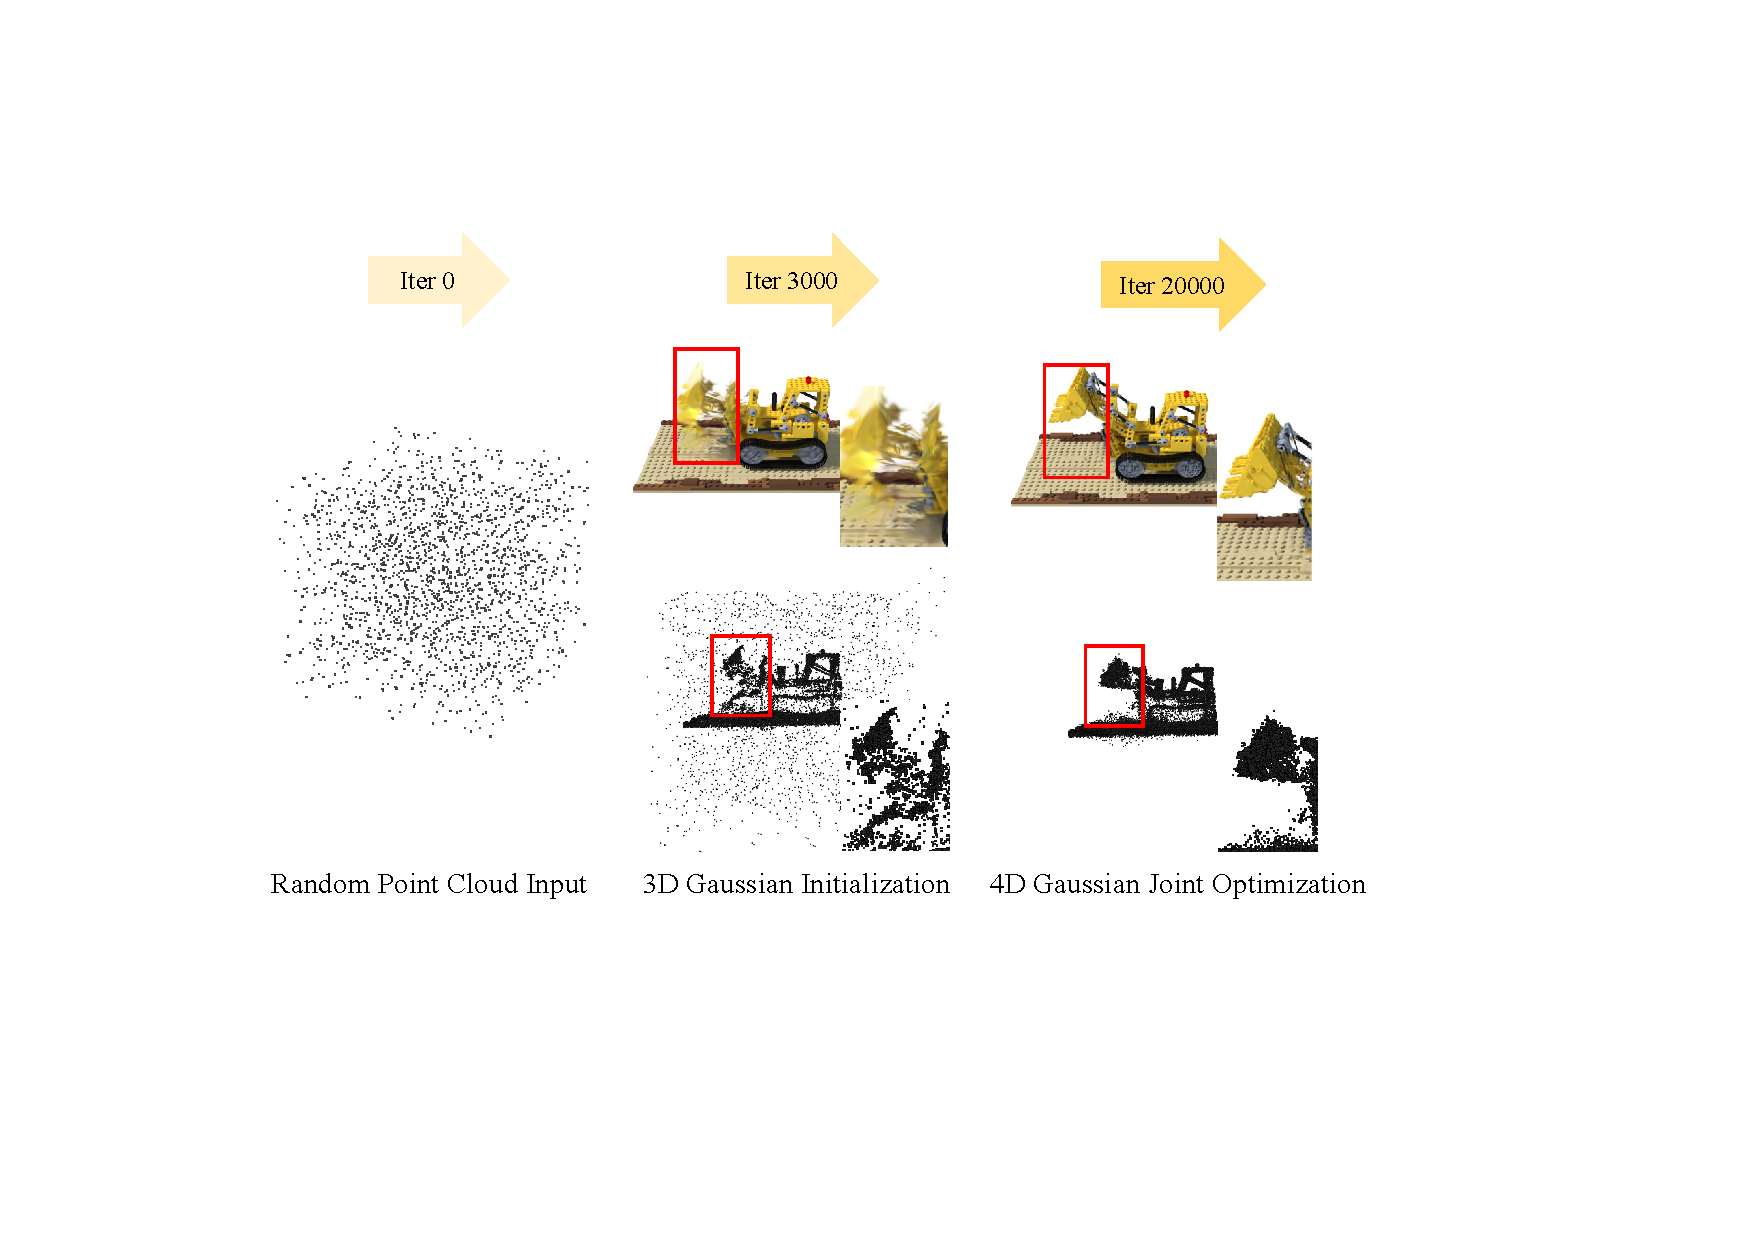
\includegraphics[width=\textwidth]{coarse2fine}
    \caption{Quá trình tối ưu coarse-to-fine: khởi tạo bằng Gaussian tĩnh giúp mô
    hình học tốt phần chuyển động. (Nguồn: bài báo gốc~\cite{wu20244dgs}.)}
    \label{fig:coarse2fine}
\end{figure}

% ============================================================
% CHƯƠNG 3 — THỰC NGHIỆM
% ============================================================
\chapter{Kết quả thực nghiệm}
\label{chap:exp}

Nhóm đã chạy lại (reproduce) toàn bộ pipeline của bài báo bằng mã nguồn chính
thức\footnote{\url{https://github.com/hustvl/4DGaussians}} trên Google Colab.

\section{Môi trường, dữ liệu và quy trình áp dụng}

\begin{itemize}
    \item \textbf{Phần cứng}: GPU NVIDIA Tesla T4 16GB (Google Colab).
    \item \textbf{Phần mềm}: Python 3.12, PyTorch 2.x, CUDA 12 (toolchain mặc định của Colab 2026).
    \item \textbf{Dữ liệu} (ba bộ, trải từ tổng hợp đến thật phản chiếu):
    \begin{itemize}
        \item \textbf{D-NeRF}~\cite{pumarola2021dnerf}: 8 cảnh động \textit{tổng hợp} đơn camera, $800\times800$ (bộ chính bài báo dùng).
        \item \textbf{HyperNeRF}~\cite{park2021hypernerf} (vrig): 4 cảnh \textit{thật} quay đa góc, $960\times540$ (bài báo cũng đánh giá).
        \item \textbf{NeRF-DS}~\cite{yan2023nerfds}: 7 cảnh \textit{thật, vật phản chiếu}, $480\times270$; \textbf{dataset ngoài bài báo}, dùng kiểm tổng quát hóa (mục~\ref{sec:nerfds}).
    \end{itemize}
    \item \textbf{Cấu hình}: đúng cấu hình gốc từng bộ: coarse 3.000 + fine 20.000 vòng (D-NeRF), coarse 3.000 + fine 14.000 (HyperNeRF, NeRF-DS).
\end{itemize}

Mã nguồn 4D-GS viết cho toolchain 2023 nên không chạy thẳng trên Colab 2026. Thay
vì vá thủ công lúc chạy, nhóm chuẩn bị sẵn một bản
fork\footnote{\url{https://github.com/MinhThang1009/4D-Gaussian}} chỉ chỉnh
\textit{tương thích môi trường} rồi clone về dùng: thay
\texttt{mmcv}$\to$\texttt{mmengine} (mmcv 1.x không build được trên Python 3.12),
bỏ ghim phiên bản \texttt{torch}/\texttt{argparse}, đổi font mặc định, vendoring
sẵn hai CUDA submodule, và đưa tỉ lệ downscale thành tham số cấu hình được
(lý do ở mục~\ref{sec:nerfds}). Để bảo đảm tính khoa học, nhóm đối chiếu trực tiếp
fork với repo gốc \texttt{hustvl/4DGaussians}: khác
biệt chỉ gồm chín tệp môi trường nói trên cộng định dạng tự động, \textbf{không
một tham số thuật toán, số vòng lặp hay hàm mất mát nào thay đổi}, nên mọi số
liệu dưới đây phản ánh đúng phương pháp gốc, chỉ khác phiên bản thư viện.

\section{Kết quả reproduce và đối sánh với bài báo}

Bảng~\ref{tab:reproduce} đối sánh kết quả nhóm chạy được (đo bằng
công cụ đánh giá chính thức tại vòng lặp 20.000) với số liệu công bố trong
bài báo trên cùng bộ dữ liệu.

\begin{table}[H]
\centering
\small
\caption{Kết quả reproduce trên 8 cảnh D-NeRF (test set) so với số liệu bài báo.}
\label{tab:reproduce}
\setlength{\tabcolsep}{5pt}
\begin{tabular}{l|cc|cc|c}
\hline
\multirow{2}{*}{\textbf{Cảnh}} & \multicolumn{2}{c|}{\textbf{PSNR (dB)}}
    & \multicolumn{2}{c|}{\textbf{SSIM}} & \textbf{FPS} \\
 & Nhóm (T4) & Bài báo & Nhóm (T4) & Bài báo & (T4) \\
\hline
bouncingballs & \textbf{40,71} & 40,62 & \textbf{0,9943} & 0,9942 & 38,2 \\
hellwarrior   & \textbf{28,79} & 28,71 & \textbf{0,9735} & 0,9733 & 33,4 \\
hook          & \textbf{32,82} & 32,73 & 0,9758 & 0,9760 & 38,5 \\
jumpingjacks  & 35,33 & 35,42 & 0,9856 & 0,9857 & 43,9 \\
lego          & \textbf{25,04} & 25,03 & 0,9376 & 0,9376 & 30,5 \\
mutant        & 37,47 & 37,59 & 0,9879 & 0,9880 & 42,1 \\
standup       & 38,11 & 38,11 & 0,9898 & 0,9898 & 41,9 \\
trex          & 34,20 & 34,23 & 0,9849 & 0,9850 & 38,2 \\
\hline
\textbf{Trung bình} & \textbf{34,06} & \textbf{34,06} & \textbf{0,9787} & \textbf{0,9787} & 38,3 \\
\hline
\end{tabular}
\end{table}

\textbf{Nhận xét}: PSNR trung bình 8 cảnh của nhóm \textbf{trùng khớp số liệu bài
báo (34,06 dB)}; từng cảnh chênh trong khoảng $\pm$0,12 dB, là mức nhiễu bình thường
do khởi tạo ngẫu nhiên (point cloud khởi tạo 2.000 điểm ngẫu nhiên, không cố định
seed) và tính không tất định của phép cộng atomic trên GPU. Kết luận: bài báo
\textbf{reproduce được}. Tốc độ render đạt $\sim$30--44 FPS trên T4, thấp hơn con số
82 FPS của bài báo do T4 yếu hơn đáng kể RTX 3090, nhưng vẫn xác nhận tính chất
thời gian thực.

Hình~\ref{fig:render_vs_gt} đối chiếu render với ground-truth ở cận cảnh trên hai
cảnh ở hai đầu thang chất lượng: \textit{mutant} (cao nhất nhóm) và \textit{lego}
(khó nhất). Mức sai khác trực quan giữa hai cảnh phản ánh đúng chênh lệch PSNR của chúng.

\begin{figure}[H]
    \centering
    \begin{minipage}{0.42\textwidth}
        \centering
        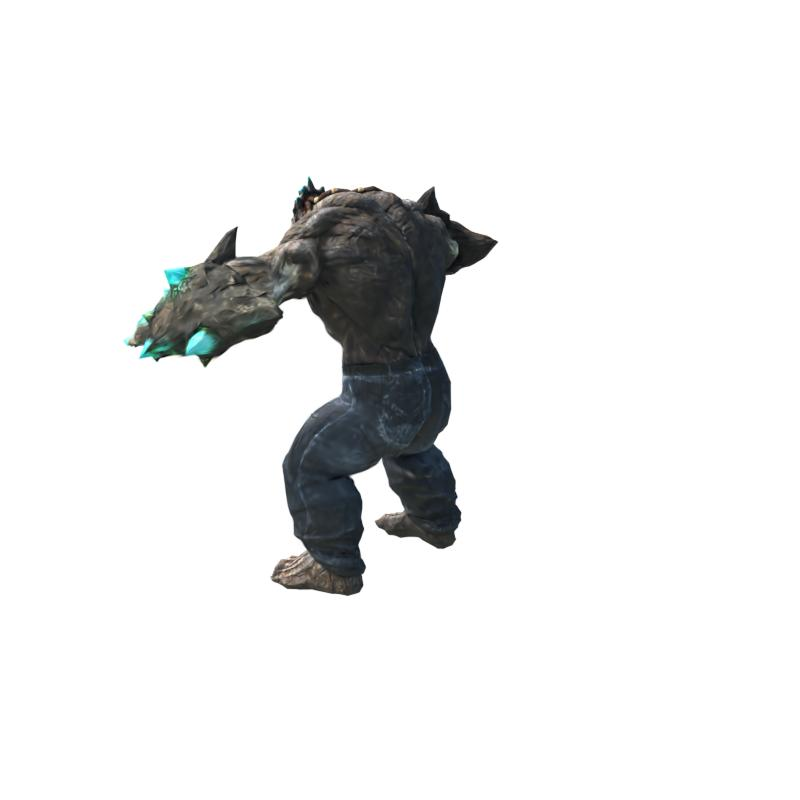
\includegraphics[width=\textwidth]{mutant_render}
        \par\small (a) Render: mutant
    \end{minipage}\hfill
    \begin{minipage}{0.42\textwidth}
        \centering
        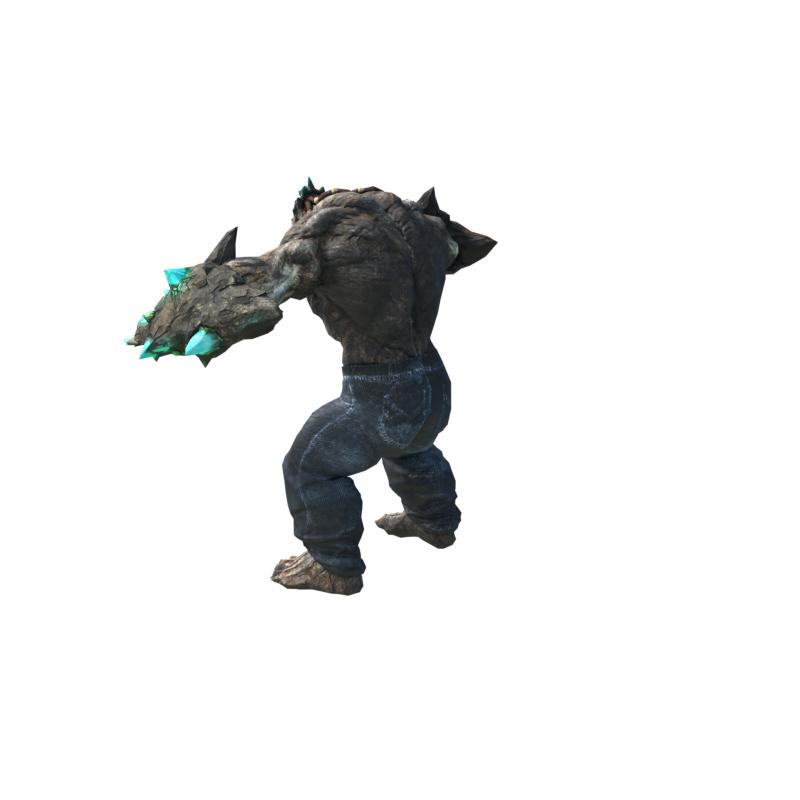
\includegraphics[width=\textwidth]{mutant_gt}
        \par\small (b) Ground-truth: mutant
    \end{minipage}

    \vspace{6pt}
    \begin{minipage}{0.42\textwidth}
        \centering
        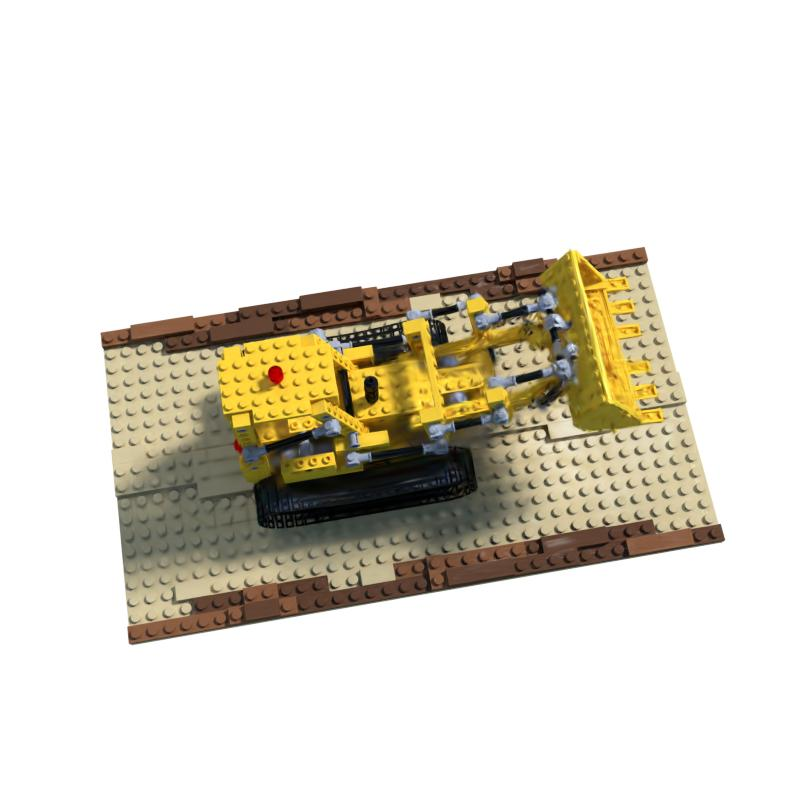
\includegraphics[width=\textwidth]{lego_render}
        \par\small (c) Render: lego
    \end{minipage}\hfill
    \begin{minipage}{0.42\textwidth}
        \centering
        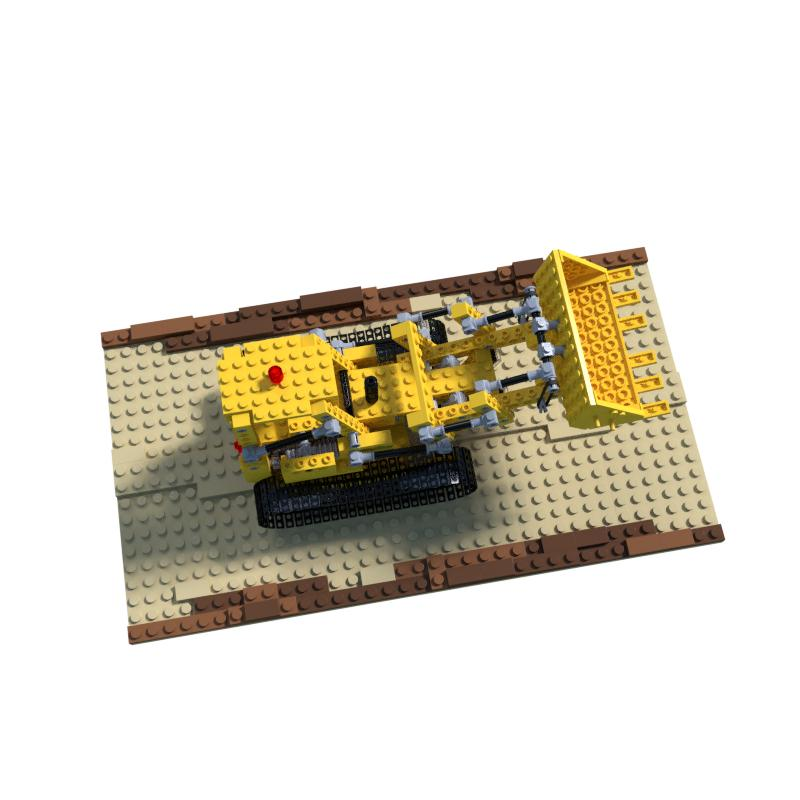
\includegraphics[width=\textwidth]{lego_gt}
        \par\small (d) Ground-truth: lego
    \end{minipage}
    \caption{So sánh ảnh render của mô hình nhóm huấn luyện với ground-truth trên
    tập test. Cảnh \textit{mutant} (37,47 dB) gần như không phân biệt được bằng mắt;
    cảnh \textit{lego} (25,04 dB), cảnh khó nhất của D-NeRF, vẫn còn sai khác
    nhỏ ở vùng chi tiết.}
    \label{fig:render_vs_gt}
\end{figure}

Hình~\ref{fig:convergence} vẽ tiến trình hội tụ của cả 8 cảnh từ log huấn luyện
của nhóm. Đường cong xác nhận trực quan tuyên bố ``hội tụ nhanh'' của bài báo:
phần lớn chất lượng đạt được ngay trong 7.000 vòng lặp đầu của giai đoạn fine
(tương đương 5--7 phút trên T4), đoạn sau chỉ tinh chỉnh thêm 1--5 dB. Biểu đồ
cũng làm lộ hai ngoại lệ có ý nghĩa: cảnh \textit{lego} chững lại rất sớm ở mức
25 dB, củng cố nhận định rằng giới hạn của cảnh này nằm ở dữ liệu (tập test lệch
phân phối so với tập train) chứ không phải ở số vòng lặp; còn \textit{hellwarrior}
cũng xuất phát ở nhóm thấp nhất đầu giai đoạn fine ($\sim$24,6 dB tại mốc 3.000)
nhưng khác \textit{lego}, nó vẫn leo đều lên gần 29 dB, cho thấy cảnh chuyển động
nhân vật mạnh cần thêm vòng lặp để hội tụ, đúng vùng nhạy cảm mà mục Limitations
của bài báo cảnh báo.

\begin{figure}[H]
    \centering
    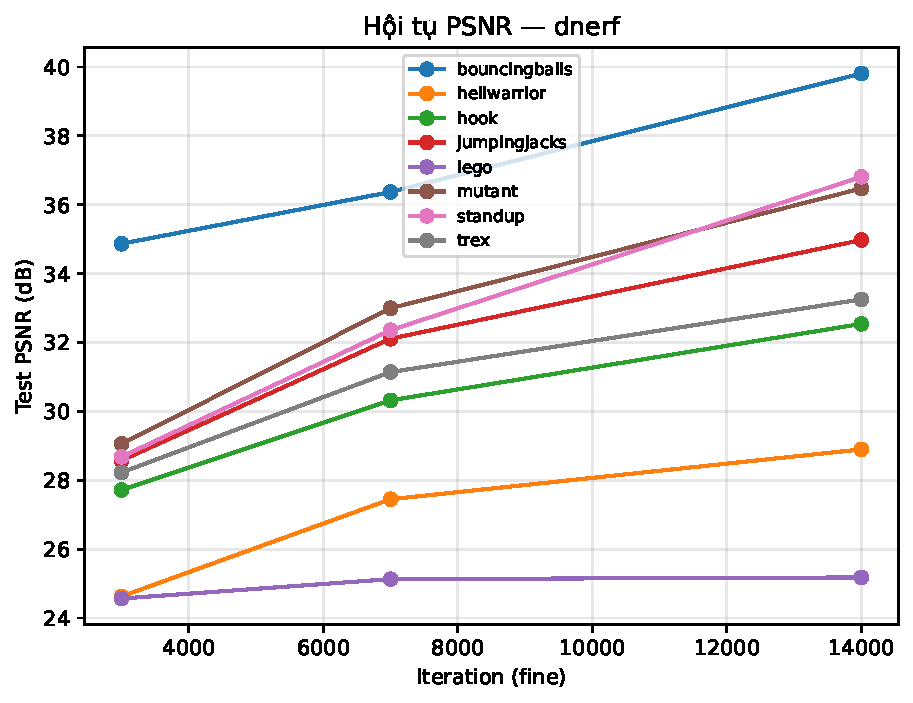
\includegraphics[width=\textwidth]{convergence_dnerf}
    \caption{Tiến trình PSNR test của 8 cảnh D-NeRF theo vòng lặp giai đoạn fine
    (eval tại 3.000/7.000/14.000). Số liệu lấy từ log huấn luyện (tensorboard, trên
    tập test lấy mẫu) nên dùng để đọc xu hướng hội tụ; giá trị tuyệt đối có thể lệch
    nhẹ so với số \texttt{metrics.py} ở bảng per-scene. Mỗi đường hội tụ về mức PSNR
    riêng theo độ khó cảnh nên các đường không gặp nhau tại một điểm. Đường dừng ở
14.000 vì test-eval chỉ log tới mốc này, dù giai đoạn fine huấn luyện tới 20.000.}
    \label{fig:convergence}
\end{figure}

Hình~\ref{fig:montage_dnerf} mở rộng đối chiếu ra toàn bộ 8 cảnh D-NeRF: ở quy mô
này hàng render gần như trùng khít hàng ground-truth, sai khác chỉ lộ ở vùng chi
tiết của cảnh khó như \textit{lego}.

\begin{figure}[H]
    \centering
    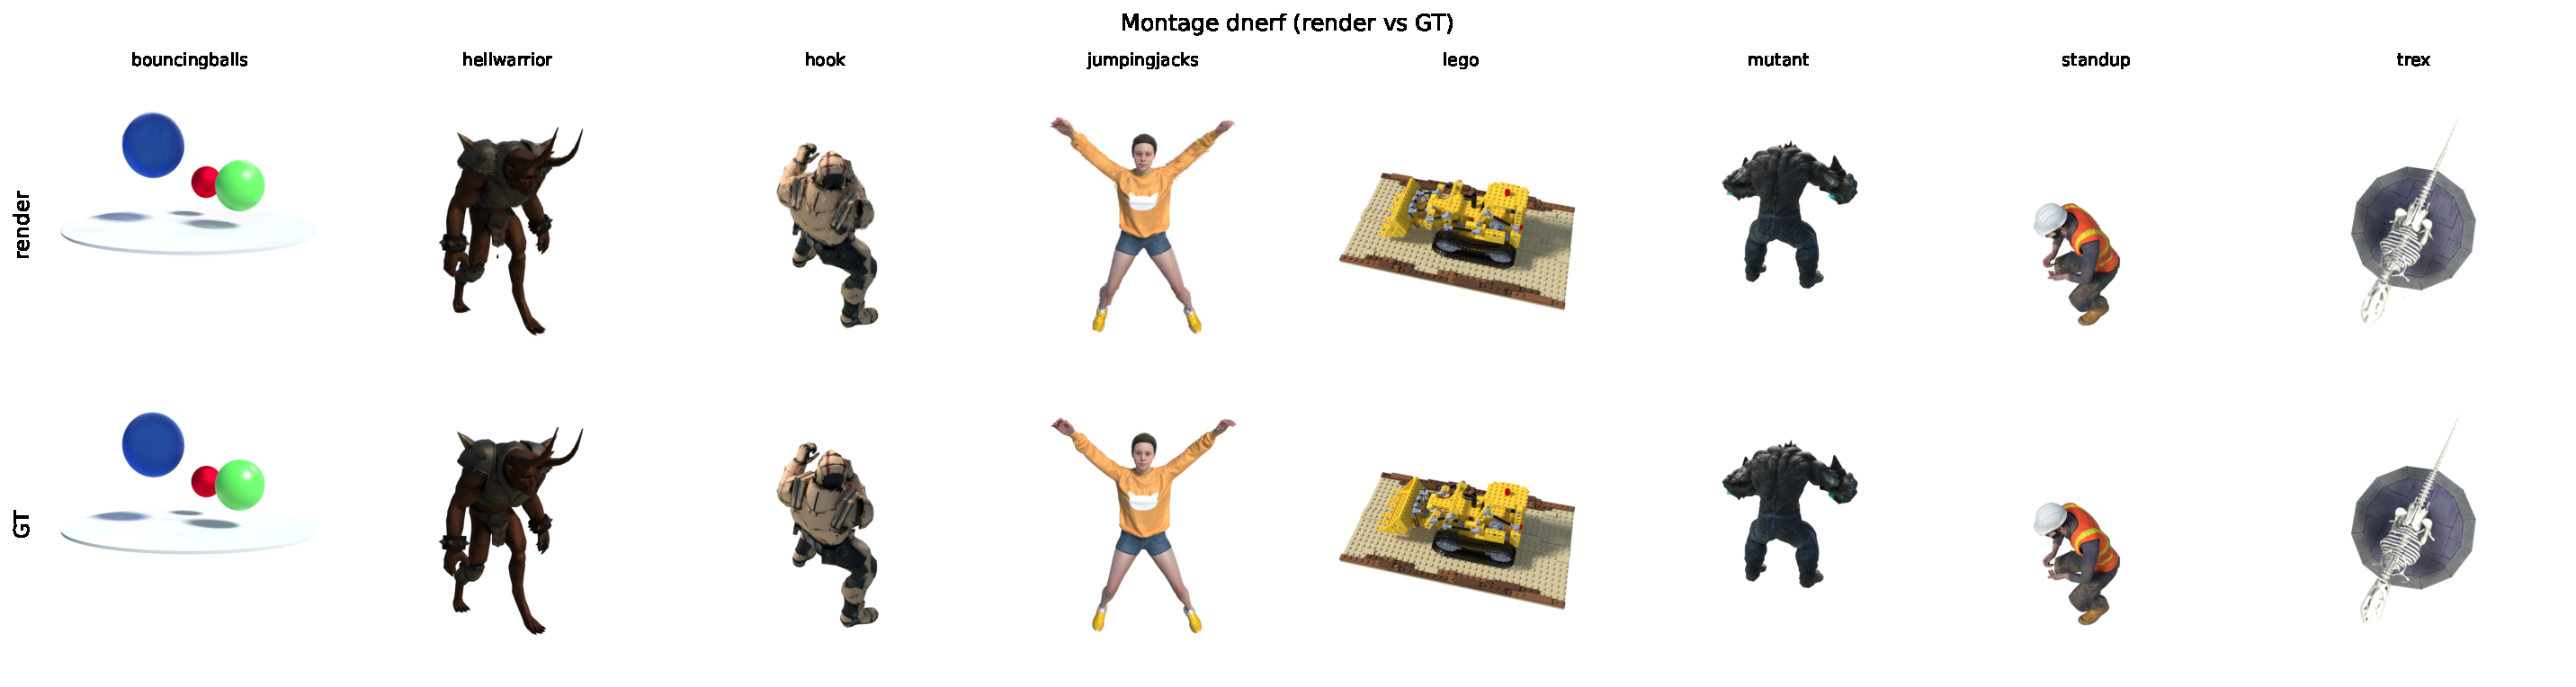
\includegraphics[width=\textwidth]{montage_dnerf}
    \caption{D-NeRF: render (hàng trên) so với ground-truth (hàng dưới) trên cả 8 cảnh test.}
    \label{fig:montage_dnerf}
\end{figure}

\section{Reproduce trên HyperNeRF (dữ liệu thật)}
\label{sec:hypernerf}

Để củng cố kết luận tái lập trên một bộ \textit{thật} chứ không chỉ tổng hợp, nhóm
chạy thêm 4 cảnh vrig của HyperNeRF~\cite{park2021hypernerf}. Khác D-NeRF, HyperNeRF
cần point cloud khởi tạo từ COLMAP; nhóm dùng bản point cloud dựng sẵn do chính tác
giả 4D-GS cung cấp để bỏ bước COLMAP nặng, giữ nguyên cấu hình
riêng cho từng cảnh của HyperNeRF (fine 14.000 vòng, tỉ lệ downscale 0,5 ứng với
ảnh ở nửa độ phân giải). Theo quy ước HyperNeRF, chất lượng đo bằng PSNR và MS-SSIM. Bài
báo chỉ công bố con số \textit{trung bình} trên tập vrig nên Bảng~\ref{tab:hypernerf}
đối sánh ở mức trung bình.

\begin{table}[H]
\centering
\small
\caption{Reproduce trên 4 cảnh vrig HyperNeRF (test set, 14.000 vòng) so với số
trung bình công bố trong bài báo~\cite{wu20244dgs} (Bảng vrig: PSNR 25,2 / MS-SSIM 0,845).}
\label{tab:hypernerf}
\setlength{\tabcolsep}{6pt}
\begin{tabular}{l|cc|c}
\hline
\textbf{Cảnh} & \textbf{PSNR (dB)} & \textbf{MS-SSIM} & \textbf{FPS (T4)} \\
\hline
3dprinter & 22,03 & 0,808 & 7,2 \\
broom2    & 21,92 & 0,687 & 8,1 \\
chicken   & 28,70 & 0,931 & 8,1 \\
banana    & 27,89 & 0,939 & 23,4 \\
\hline
\textbf{Trung bình (nhóm)} & \textbf{25,13} & \textbf{0,841} & 11,7 \\
\textbf{Bài báo (RTX 3090)} & 25,2 & 0,845 & 34 \\
\hline
\end{tabular}
\end{table}

\textbf{Nhận xét}: PSNR trung bình của nhóm \textbf{25,13 dB} và MS-SSIM \textbf{0,841}
bám sát số công bố 25,2 / 0,845 (lệch lần lượt chỉ $-0{,}07$ dB và $-0{,}004$).
Là dữ liệu thật đơn camera nhiễu hơn D-NeRF, HyperNeRF thường khó tái lập sát tuyệt
đối hơn cảnh tổng hợp; điểm cần khẳng định là kết quả nằm trong vùng sai số hợp lý
quanh số công bố, qua đó xác nhận pipeline chạy đúng trên \textit{cả} dữ liệu tổng
hợp lẫn thật trước khi mở rộng sang dataset ngoài bài báo (mục~\ref{sec:nerfds}).

Hình~\ref{fig:montage_hypernerf} đặt render cạnh ground-truth trên cả 4 cảnh vrig:
mô hình bám sát ảnh thật ở cảnh giàu kết cấu (chicken, banana), sai khác rõ hơn ở
cảnh khó \textit{broom2}.

\begin{figure}[H]
    \centering
    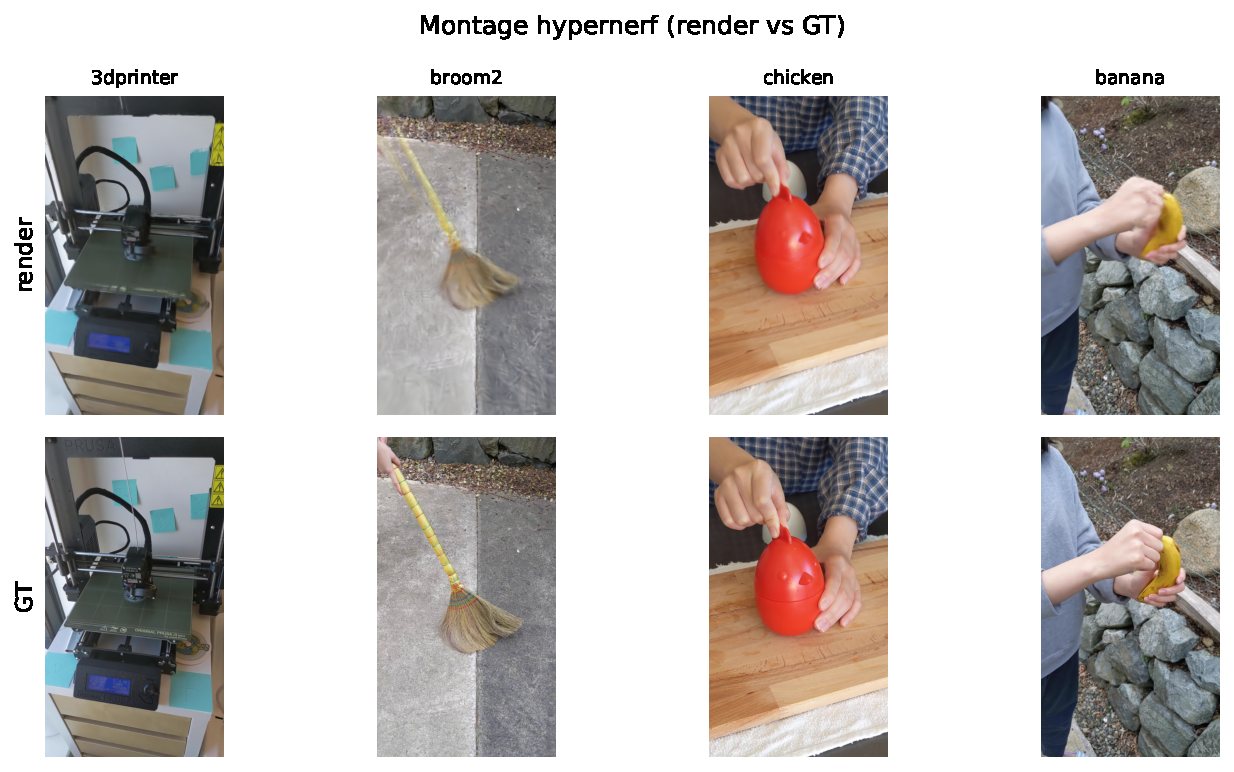
\includegraphics[width=\textwidth]{montage_hypernerf}
    \caption{HyperNeRF: render (hàng trên) so với ground-truth (hàng dưới) trên 4 cảnh vrig.}
    \label{fig:montage_hypernerf}
\end{figure}

Hình~\ref{fig:conv_hypernerf} vẽ tiến trình hội tụ PSNR test của 4 cảnh và tách
thành hai nhóm rõ rệt: chicken và banana (tiền cảnh rõ, giàu kết cấu) leo đều qua
cả ba mốc eval và vẫn còn cải thiện ở vòng 14.000, trong khi 3dprinter và broom2
bão hòa quanh 22 dB ngay từ đầu giai đoạn fine rồi gần như đi ngang. Trần chất
lượng của hai cảnh sau vì thế bị giới hạn bởi độ khó dữ liệu (broom2 là cảnh khó
nhất bộ, chỉ số cấu trúc thấp) chứ không phải số vòng lặp.

\begin{figure}[H]
    \centering
    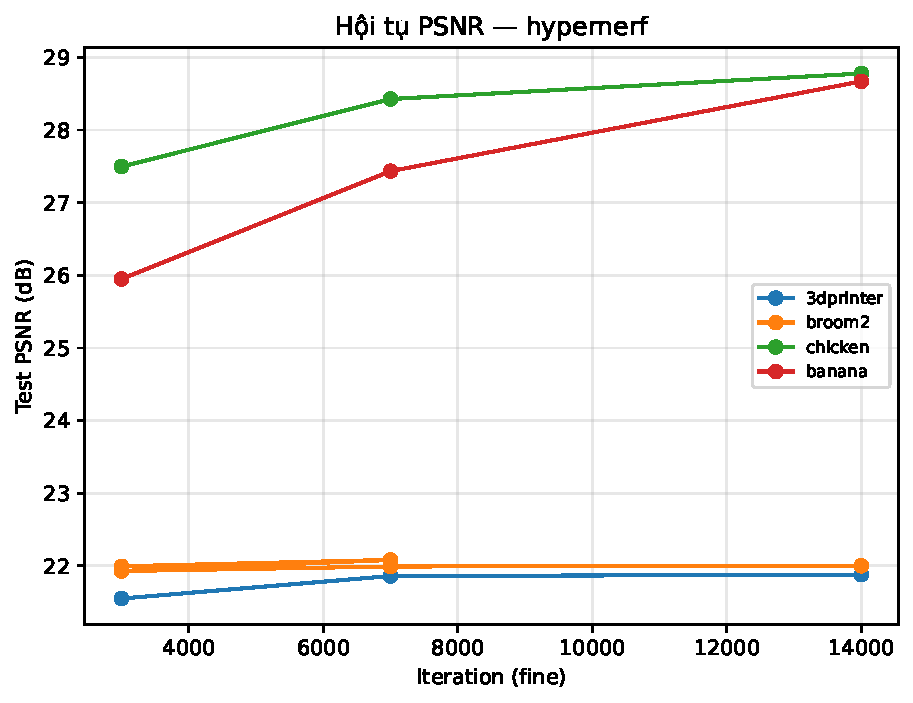
\includegraphics[width=\textwidth]{convergence_hypernerf}
    \caption{Tiến trình PSNR test của 4 cảnh HyperNeRF theo vòng lặp giai đoạn fine
    (eval tại 3.000/7.000/14.000). Số liệu từ log huấn luyện (tensorboard, tập test
    lấy mẫu), dùng đọc xu hướng; có thể lệch nhẹ so với số \texttt{metrics.py} ở bảng per-scene.}
    \label{fig:conv_hypernerf}
\end{figure}

\section{So sánh với các phương pháp khác}

Bảng~\ref{tab:sota} trích số liệu trung bình trên D-NeRF từ bài báo, bổ sung cột
kết quả reproduce của nhóm.

\begin{table}[H]
\centering
\small
\caption{So sánh các phương pháp trên bộ D-NeRF ($800\times800$), số liệu trích từ
bài báo~\cite{wu20244dgs}. ``Time'' là thời gian huấn luyện. Ô \colorbox{red!25}{hồng}
= tốt nhất, \colorbox{yellow!25}{vàng} = nhì (xét trong các phương pháp công bố; dòng
4D-GS của nhóm là tái lập, không tính xếp hạng).}
\label{tab:sota}
\setlength{\tabcolsep}{4.5pt}
\resizebox{\textwidth}{!}{%
\begin{tabular}{l|ccc|c|cc}
\hline
\textbf{Phương pháp} & \textbf{PSNR (dB)}$\uparrow$ & \textbf{SSIM}$\uparrow$
    & \textbf{LPIPS}$\downarrow$ & \textbf{Time}$\downarrow$
    & \textbf{FPS}$\uparrow$ & \textbf{Storage (MB)}$\downarrow$ \\
\hline
TiNeuVox-B~\cite{tineuvox}   & 32,67 & 0,97 & 0,04 & 28 phút  & 1,5  & 48 \\
K-Planes~\cite{kplanes}      & 31,61 & 0,97 & --   & 52 phút  & 0,97 & 418 \\
HexPlane-Slim~\cite{hexplane}& 31,04 & 0,97 & 0,04 & 11,5 phút & 2,5  & 38 \\
3D-GS~\cite{3dgs}            & 23,19 & 0,93 & 0,08 & \cellcolor{yellow!25}10 phút  & \cellcolor{red!25}170 & \cellcolor{red!25}10 \\
FFDNeRF~\cite{guo2023forwardflowfornvs} & \cellcolor{yellow!25}32,68 & 0,97 & 0,04 & -- & $<$1 & 440 \\
MSTH~\cite{msth}             & 31,34 & \cellcolor{yellow!25}0,98 & \cellcolor{yellow!25}0,02 & \cellcolor{red!25}6 phút & -- & -- \\
\hline
4D-GS (bài báo, RTX 3090)    & \cellcolor{red!25}34,05 & \cellcolor{red!25}0,98 & \cellcolor{red!25}0,02 & 20 phút & \cellcolor{yellow!25}82 & \cellcolor{yellow!25}18 \\
4D-GS (nhóm, Colab T4)       & 34,06 & 0,98 & 0,03 & $\sim$13,5 phút & 38,3 & $\approx$24,8 \\
\hline
\end{tabular}%
}
\end{table}

4D-GS dẫn đầu về chất lượng (cao hơn TiNeuVox-B 1,4 dB) trong khi render nhanh
hơn các phương pháp NeRF-based 30--85 lần; 3D-GS tĩnh tuy render nhanh nhất nhưng
hoàn toàn thất bại với cảnh động (23,19 dB) vì không mô hình hóa chuyển động.
Lưu ý nhỏ về làm tròn: bảng tổng của bài báo in 34,05 dB, trong khi trung bình
tính từ bảng per-scene của chính bài báo là 34,06 dB (Bảng~\ref{tab:reproduce});
hai con số là một, khác nhau ở bước làm tròn của tác giả.

\section{Tổng quát hóa trên dataset ngoài bài báo: NeRF-DS}
\label{sec:nerfds}

\subsection*{Lựa chọn dataset và phân tích điều kiện áp dụng}

Để kiểm tra khả năng tổng quát hóa, nhóm áp dụng nguyên thuật toán lên
\textbf{NeRF-DS}~\cite{yan2023nerfds}: bộ dữ liệu thật đơn camera quay các
\textit{vật thể phản chiếu chuyển động} (rây inox, đĩa men bóng, ấm kim loại)
mà bài báo gốc \textbf{không} đánh giá. Lựa chọn này có chủ đích kép: NeRF-DS
vừa nằm ngoài các benchmark tác giả tự chọn, vừa tấn công thẳng vào giả định mà
nhóm nhận diện được khi đọc phương pháp (mục~\ref{sec:deform}): màu Gaussian là hệ số SH
\textit{cố định theo thời gian}, còn bộ giải mã chỉ biến dạng vị trí và hình
dạng. Trên vật thể bóng đang chuyển động, vệt phản xạ trượt trên bề mặt theo
thời gian, tức là một hiệu ứng \textit{quang học} chứ không phải \textit{hình
học}; theo phân tích này, nhóm \textbf{dự đoán trước} rằng 4D-GS sẽ đạt kết quả
khá trên cảnh hình học chiếm ưu thế nhưng suy giảm rõ trên cảnh phản xạ chiếm
ưu thế.

Việc áp dụng bắt đầu từ ``hợp đồng đầu vào'' của mã nguồn: thuật toán cần (i)
ảnh kèm camera pose và nhãn thời gian theo định dạng Nerfies/HyperNeRF, (ii)
một point cloud khởi tạo, và (iii) một file cấu hình khớp đặc tính dữ liệu.
NeRF-DS được xây trên chính toolchain Nerfies nên điều kiện (i) thỏa mãn ngay,
bộ nạp dữ liệu kiểu HyperNeRF của mã nguồn đọc được không cần sửa. Với (iii), nhóm
tái dùng thiết lập mặc định của HyperNeRF vì NeRF-DS tương đồng về mọi đặc tính mà
cấu hình mã hóa: video thật đơn camera, vài trăm khung hình, độ phân giải thấp. Chỉ điều kiện (ii) bị thiếu: tác giả 4D-GS cung cấp point
cloud COLMAP dựng sẵn cho HyperNeRF nhưng dĩ nhiên không có cho NeRF-DS.

\subsection*{Các điều chỉnh kỹ thuật}

Thay vì chạy lại toàn bộ pipeline COLMAP dense (nhiều giờ trên Colab), nhóm tận
dụng đám mây điểm 3D có sẵn của NeRF-DS, vốn sinh ra từ chính bước đăng ký camera
của bộ dữ liệu nên \textit{cùng hệ tọa độ thế giới} với các pose, và chuyển sang
định dạng point cloud mà bộ nạp yêu cầu (32.143 điểm cho cảnh \textit{sieve},
9.714 điểm cho \textit{plate}). Đây là khởi tạo hình
học hợp lệ về nguyên tắc, dù thưa hơn COLMAP dense; cơ chế densification của
3D-GS (mục~\ref{sec:3dgs}) sau đó tự tăng mật độ lên khoảng 40.000--86.000 điểm tùy cảnh trong
quá trình huấn luyện, xác nhận khởi tạo thưa được bù đắp.

Điều chỉnh thứ hai phát hiện qua một lỗi chạy: công cụ đánh giá chính thức báo ảnh
quá nhỏ cho phép đo MS-SSIM. Truy ngược, nhóm thấy bộ đọc dữ liệu của mã nguồn
\textit{cố định cứng} tỉ lệ downscale $0{,}5$; với HyperNeRF (ảnh gốc lớn) giá trị
này vô hại, nhưng ảnh NeRF-DS gốc chỉ $480\times270$ nên bị giảm còn $240\times135$,
vừa gây lỗi đo vừa thổi phồng PSNR (ảnh nhỏ dễ đạt điểm cao). Trong bản fork, nhóm tách tỉ lệ này thành
tham số cấu hình được\footnote{Cụ thể là biến môi trường \texttt{HYPER\_RATIO}; chi
tiết tại repository mã nguồn của nhóm.} và đặt $1{,}0$ cho NeRF-DS, rồi
huấn luyện lại từ đầu để mọi con số trong Bảng~\ref{tab:nerfds} được đo ở đúng độ
phân giải gốc, bảo đảm so sánh công bằng với số liệu bên thứ ba
(SpectroMotion~\cite{spectromotion}).

\subsection*{Kết quả và kiểm chứng dự đoán}

\begin{table}[H]
\centering
\small
\caption{4D-GS trên 7 cảnh NeRF-DS (test set, $480\times270$, 14.000 vòng): số nhóm
tự đo bằng công cụ đánh giá chính thức, đặt cạnh số 4D-GS trong bảng baseline của
SpectroMotion~\cite{spectromotion} (CVPR 2025), vì bài báo 4D-GS gốc không đánh
giá NeRF-DS. LPIPS đều là biến thể VGG. Số PSNR in đậm là cảnh nhóm vượt SpectroMotion.}
\label{tab:nerfds}
\setlength{\tabcolsep}{5pt}
\begin{tabular}{l|ccc|c|c}
\hline
\textbf{Cảnh} & \textbf{PSNR nhóm} & \textbf{SSIM nhóm} & \textbf{LPIPS nhóm}
 & \textbf{PSNR~\cite{spectromotion}} & \textbf{FPS (T4)} \\
\hline
as    & \textbf{25,68} & 0,8711 & 0,1893 & 24,85 & 104,6 \\
basin & 19,17 & 0,7669 & 0,2276 & 19,26 & 79,3 \\
bell  & 22,62 & 0,8127 & 0,2015 & 22,86 & 60,7 \\
cup   & \textbf{24,23} & 0,8772 & 0,1673 & 23,82 & 70,4 \\
plate & 17,81 & 0,7423 & 0,3301 & 18,77 & 93,7 \\
press & 24,10 & 0,8199 & 0,2468 & 24,82 & 85,9 \\
sieve & \textbf{25,72} & 0,8637 & 0,1688 & 25,16 & 77,0 \\
\hline
\textbf{Trung bình} & 22,76 & 0,8220 & 0,2188 & 22,79 & 81,7 \\
\hline
\end{tabular}
\end{table}

Đặt cạnh số 4D-GS bên thứ ba của SpectroMotion~\cite{spectromotion}, kết quả
per-scene của nhóm khớp sát (PSNR trung bình 22,76 so với 22,79; sai số mỗi cảnh
trung bình $\sim$0,5 dB, lớn nhất $\sim$1 dB ở \textit{plate}), xác nhận quy trình áp dụng 4D-GS lên một
dataset ngoài bài báo là đúng đắn và hành vi phương pháp ổn định khi tái lập độc
lập. Quan trọng hơn, kết quả \textbf{khớp với dự đoán lý thuyết} nhóm đặt ra trước
khi chạy, thấy rõ nhất qua hai cảnh tương phản: \textit{sieve} (rây inox, hình học
chiếm ưu thế) đạt 25,72 dB ở mức khá của bộ dữ liệu, còn \textit{plate} (đĩa men
bóng, mặt phản chiếu chiếm phần lớn khung hình) rớt xuống 17,81 dB. Quan sát ảnh
render (Hình~\ref{fig:nerfds}) cho thấy đúng cơ chế thất bại đã dự đoán: hình dạng
chiếc đĩa dựng tương đối ổn nhưng vệt phản xạ trên mặt đĩa bị nhòe thành màu trung
bình, vì mỗi Gaussian chỉ có một bộ màu SH cố định cho mọi thời điểm nên lời giải
tối ưu của nó là ``trung bình hóa'' các trạng thái phản xạ qua thời gian.

Thí nghiệm còn phơi bày một điểm yếu thứ hai: khoảng cách train-test rất lớn
(train PSNR xấp xỉ 38 dB so với test 25,72 dB trên \textit{sieve}, chênh hơn
12 dB) cho thấy
\textbf{overfitting} rõ rệt trong thiết lập đơn camera trên dữ liệu thật, nhất
quán với hiện tượng tác giả mô tả trên bộ iPhone trong phụ lục. Đặt trong bức
tranh rộng hơn, trên NeRF-DS lợi thế \textit{chất lượng} của 4D-GS gần như không
còn: trong bảng baseline NeRF-DS của SpectroMotion~\cite{spectromotion} (CVPR 2025),
4D-GS (22,79 dB) xếp sau các phương pháp chuyên cho vật phản chiếu (Deformable 3DGS~\cite{deformable3dgs}
23,43 dB và chính SpectroMotion 24,17 dB), dù vẫn vượt HyperNeRF (19,01 dB) trên cùng
bộ. Điều \textit{chắc chắn} rút ra được là 4D-GS đánh mất ưu thế chất lượng so với khi chạy trên dữ liệu
tổng hợp (D-NeRF $\sim$34 dB) hay thật khuếch tán (HyperNeRF), và trên dữ liệu phản
chiếu thế mạnh còn lại chủ yếu là tốc độ render. Cả hai phát hiện (giới hạn với
vật liệu phản chiếu và overfitting đơn camera) đều không được nêu trong bài báo
gốc và sẽ được bàn tiếp ở chương~\ref{chap:critical}.

\begin{figure}[H]
    \centering
    \begin{minipage}{0.42\textwidth}
        \centering
        
\includegraphics[width=\textwidth]{sieve_render}
        \par\small (a) Render: sieve
    \end{minipage}\hfill
    \begin{minipage}{0.42\textwidth}
        \centering
        
\includegraphics[width=\textwidth]{sieve_gt}
        \par\small (b) Ground-truth: sieve
    \end{minipage}

    \vspace{6pt}
    \begin{minipage}{0.42\textwidth}
        \centering
        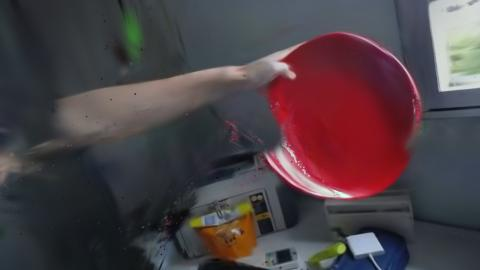
\includegraphics[width=\textwidth]{plate_render}
        \par\small (c) Render: plate
    \end{minipage}\hfill
    \begin{minipage}{0.42\textwidth}
        \centering
        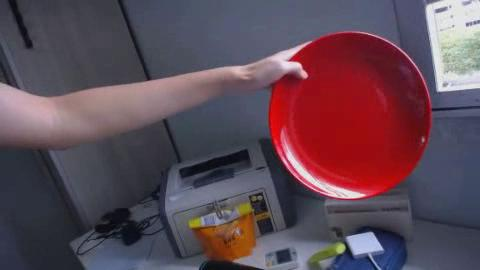
\includegraphics[width=\textwidth]{plate_gt}
        \par\small (d) Ground-truth: plate
    \end{minipage}
    \caption{Kết quả trên NeRF-DS. Cảnh \textit{sieve} (25,72 dB) giữ được hình
    học tốt; cảnh \textit{plate} (17,81 dB) mất chi tiết phản xạ trên mặt đĩa,
    minh chứng cho hạn chế với vật liệu phản chiếu.}
    \label{fig:nerfds}
\end{figure}

Hình~\ref{fig:montage_nerfds} mở rộng đối chiếu render với ground-truth ra cả 7 cảnh
NeRF-DS, cho thấy chất lượng cao ở cảnh hình học chiếm ưu thế và giảm rõ ở cảnh
phản chiếu như \textit{plate}.

\begin{figure}[H]
    \centering
    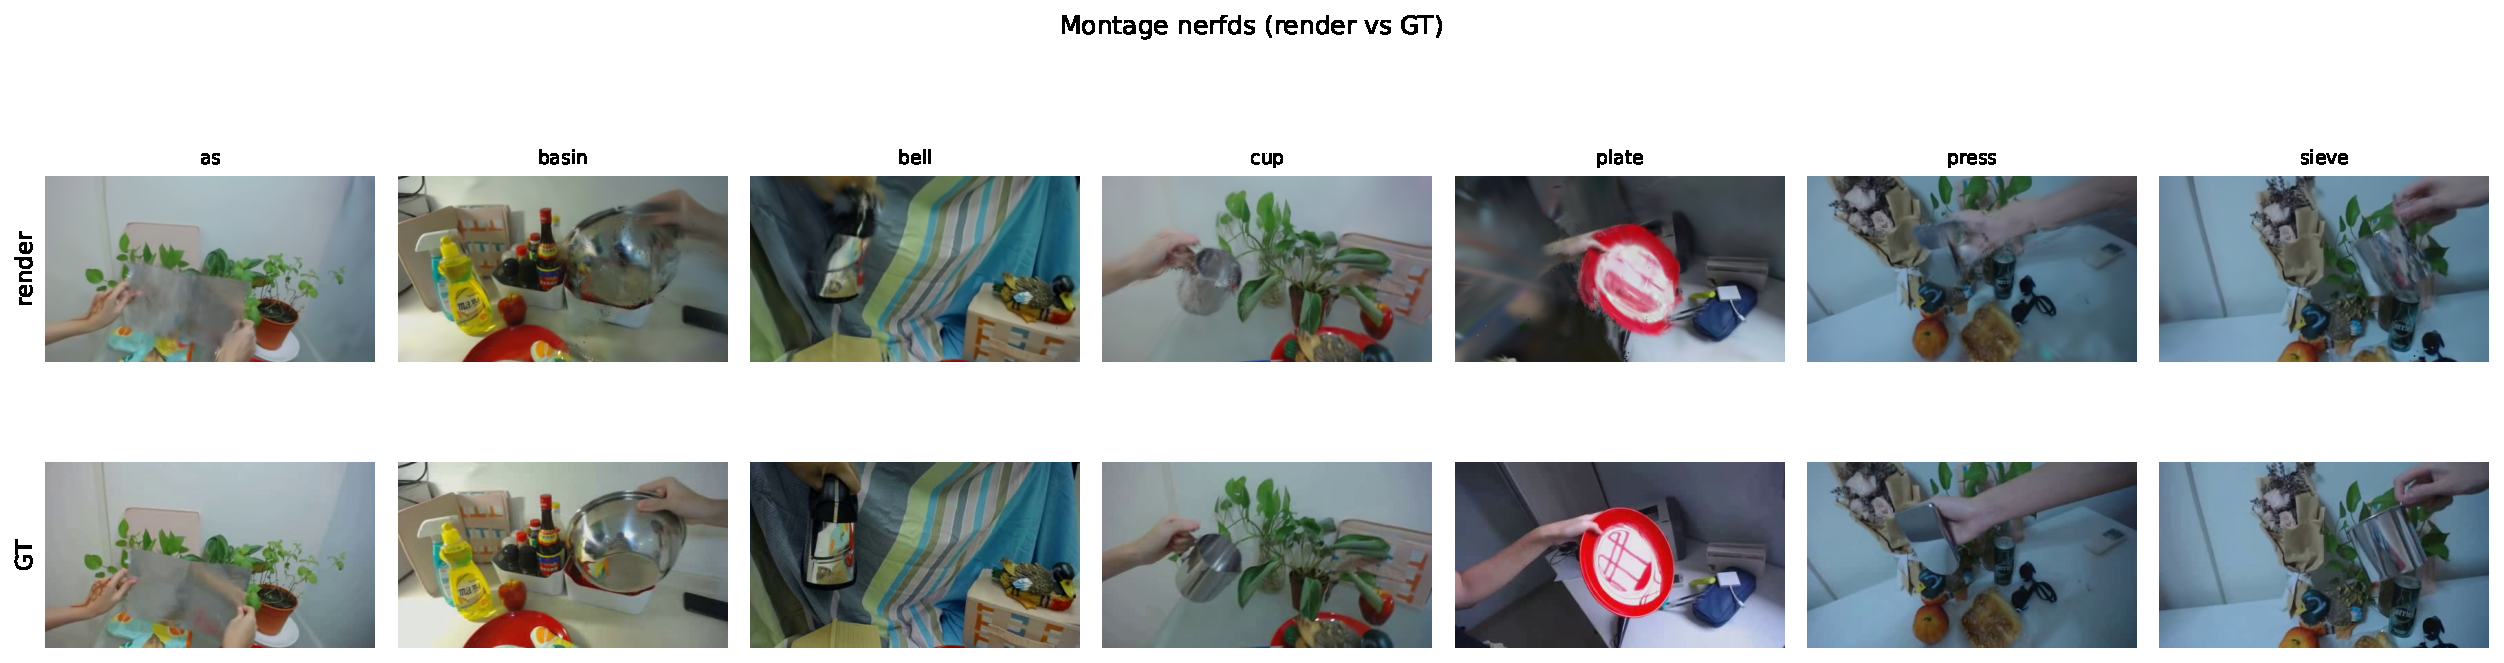
\includegraphics[width=\textwidth]{montage_nerfds}
    \caption{NeRF-DS: render (hàng trên) so với ground-truth (hàng dưới) trên cả 7 cảnh test.}
    \label{fig:montage_nerfds}
\end{figure}

Hình~\ref{fig:conv_nerfds} là tiến trình hội tụ PSNR test của 7 cảnh NeRF-DS, mỗi
cảnh bão hòa về mức PSNR riêng theo độ khó (cảnh phản chiếu \textit{plate} hội tụ ở
mức thấp nhất).

\begin{figure}[H]
    \centering
    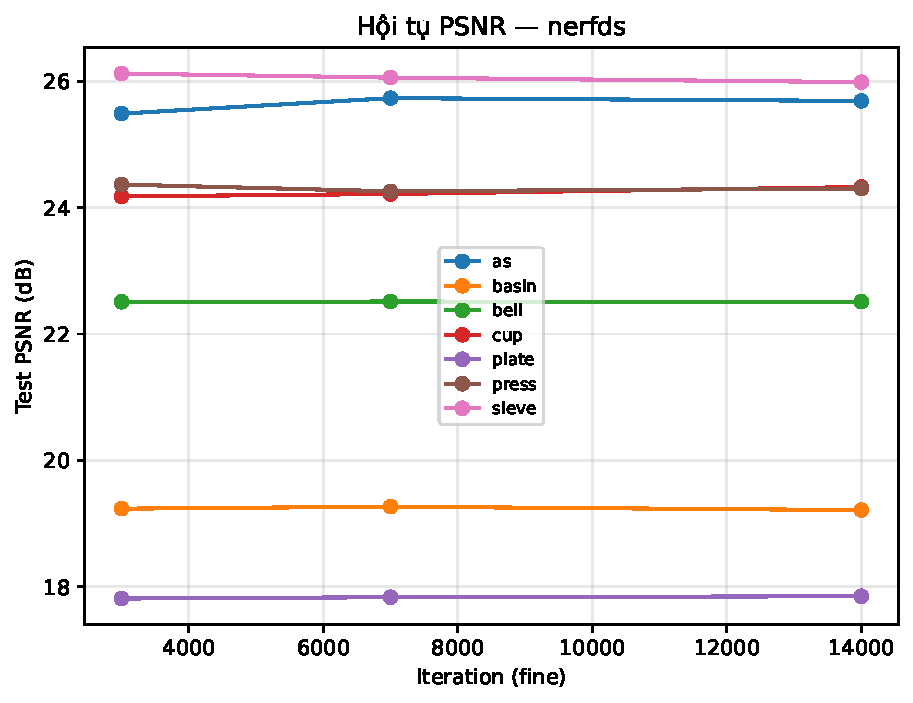
\includegraphics[width=\textwidth]{convergence_nerfds}
    \caption{Tiến trình PSNR test của 7 cảnh NeRF-DS theo vòng lặp giai đoạn fine
    (eval tại 3.000/7.000/14.000). Số liệu từ log huấn luyện (tensorboard, tập test
    lấy mẫu), dùng đọc xu hướng; có thể lệch nhẹ so với số \texttt{metrics.py} ở bảng per-scene.}
    \label{fig:conv_nerfds}
\end{figure}

Tổng kết Trục 1 (tái lập vs công bố): Hình~\ref{fig:repro_bar} đặt cạnh nhau kết quả của nhóm
và số công bố trên cả ba dataset cùng lúc. Ở mọi cặp cột (PSNR, SSIM, MS-SSIM,
LPIPS-vgg) chiều cao gần như trùng khít: chênh lệch PSNR đều dưới $0{,}1$ dB và
các chỉ số cấu trúc chỉ lệch ở hàng phần trăm. Trực quan này xác nhận một lần nữa
pipeline tái lập đúng số công bố trên cả dữ liệu tổng hợp (D-NeRF) lẫn dữ liệu
thật (HyperNeRF) lẫn dữ liệu thật phản chiếu (NeRF-DS so với SpectroMotion), tạo
nền tin cậy cho phần đối sánh chéo ngay sau đây.

\begin{figure}[H]
    \centering
    
\includegraphics[width=\textwidth]{bar_repro_vs_paper}
    \caption{Trục 1: đối sánh kết quả nhóm với số công bố trên từng dataset
    (D-NeRF: PSNR/SSIM/LPIPS; HyperNeRF: PSNR/MS-SSIM; NeRF-DS: PSNR/SSIM/LPIPS-vgg
    so SpectroMotion~\cite{spectromotion}). Cột ``Nhóm'' sát cột ``Bài báo'' xác nhận
    tái lập đúng.}
    \label{fig:repro_bar}
\end{figure}

\section{Đối sánh chéo ba dataset: hành vi của 4D-GS theo độ khó}
\label{sec:cross}

Các mục trên so từng dataset với số công bố (Trục 1, trả lời ``tái lập có đúng không'').
Mục này tổng hợp theo \textbf{Trục 2} (đối sánh chéo): đặt cùng một mô hình 4D-GS do nhóm huấn
luyện lên ba dataset cạnh nhau để đọc \textbf{hành vi của phương pháp theo độ khó
tăng dần} của dữ liệu: tổng hợp (D-NeRF) $\to$ thật khuếch tán (HyperNeRF) $\to$
thật phản chiếu (NeRF-DS). Đây là phân tích chính của báo cáo vì nó trả lời câu hỏi
mà bảng đối sánh với bài báo không trả lời: \textit{4D-GS mạnh/yếu ở loại cảnh nào}.

\begin{table}[H]
\centering
\small
\caption{4D-GS (mô hình nhóm huấn luyện) trên ba dataset, trung bình mỗi bộ. Cột
chất lượng dùng chung PSNR/SSIM/LPIPS-vgg; cột hiệu năng FPS/dung lượng/số Gaussian
là đặc tính phương pháp (so trực tiếp được, không phụ thuộc cảnh).}
\label{tab:cross}
\setlength{\tabcolsep}{5pt}
\begin{tabular}{l|c|ccc|ccc}
\hline
\textbf{Dataset} & \textbf{Loại} & \textbf{PSNR}$\uparrow$ & \textbf{SSIM}$\uparrow$
 & \textbf{LPIPS}$\downarrow$ & \textbf{FPS}$\uparrow$ & \textbf{MB}$\downarrow$ & \textbf{\#Gauss} \\
\hline
D-NeRF    & tổng hợp         & 34,06 & 0,9787 & 0,0262 & 38,3 & 24,8 & $\sim$44.900 \\
HyperNeRF & thật             & 25,13 & 0,6853 & 0,3374 & 11,7 & 70,2 & $\sim$160.400 \\
NeRF-DS   & thật, phản chiếu & 22,76 & 0,8220 & 0,2188 & 81,7 & 45,4 & $\sim$59.500 \\
\hline
\end{tabular}
\end{table}

\begin{figure}[H]
    \centering
    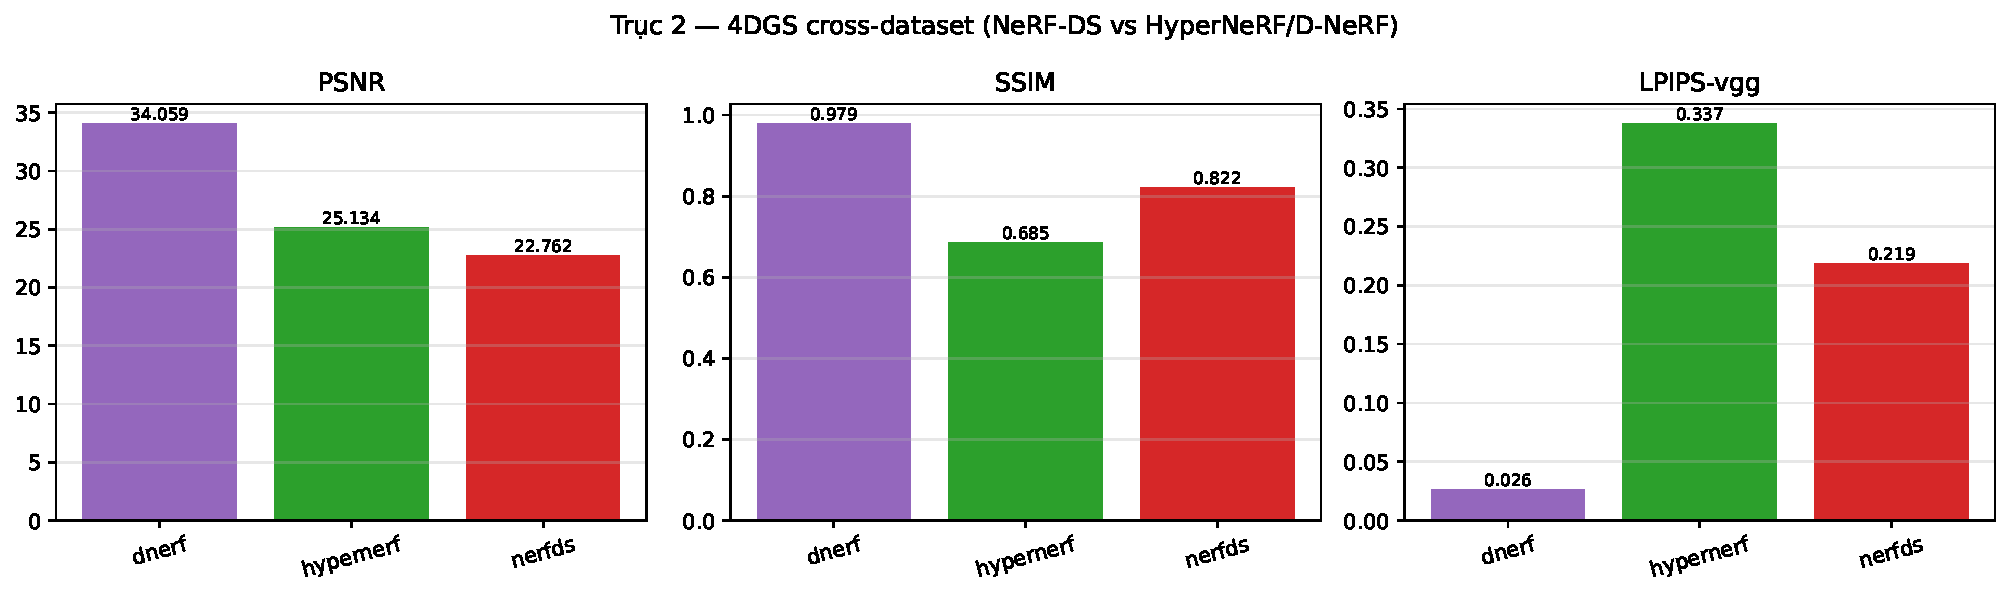
\includegraphics[width=\textwidth]{bar_cross_dataset}
    \caption{So sánh 4D-GS trên ba dataset (PSNR/SSIM/LPIPS). \textbf{PSNR} giảm dần
    theo trục tổng hợp (D-NeRF) $\to$ thật (HyperNeRF) $\to$ thật phản chiếu (NeRF-DS);
    riêng SSIM/LPIPS không đơn điệu do khác độ phân giải và cảnh (xem phần ``Đọc kết quả'').}
    \label{fig:cross}
\end{figure}

\textbf{Đọc kết quả} (Bảng~\ref{tab:cross}, trực quan ở Hình~\ref{fig:cross}): PSNR giảm dần theo độ khó của dữ liệu: D-NeRF \textbf{34,06}
$>$ HyperNeRF \textbf{25,13} $>$ NeRF-DS \textbf{22,76} dB. Tuy nhiên SSIM và LPIPS
\textit{không} theo cùng chiều: NeRF-DS (SSIM 0,8220 / LPIPS 0,2188) thậm chí nhỉnh hơn
HyperNeRF (0,6853 / 0,3374), một phần vì cảnh \textit{broom2} kéo tụt trung bình của
HyperNeRF, một phần vì NeRF-DS độ phân giải thấp hơn ($480\times270$) nên dễ đạt
SSIM/LPIPS cao, minh họa đúng cảnh báo rằng so trị tuyệt đối giữa các bộ khác độ
phân giải là không công bằng. Do đó kết luận 4D-GS suy giảm trên vật phản chiếu dựa
chủ yếu vào PSNR và đối sánh per-scene với các phương pháp chuyên specular
(mục~\ref{sec:nerfds}), không dựa SSIM/LPIPS cross-dataset.
Xu hướng kỳ vọng (cũng là luận điểm nhóm đặt ra từ phân tích phương pháp, mục~\ref{sec:deform})
là chất lượng giảm dần theo trục tổng hợp $\to$ thật $\to$ phản chiếu, trong khi
FPS, dung lượng và số Gaussian giữ ổn định. Riêng NeRF-DS tụt rõ so với HyperNeRF dù
cả hai đều là dữ liệu thật đơn camera, cô lập đúng \textit{một} biến khác biệt là vật
liệu phản chiếu, củng cố chẩn đoán ở mục~\ref{sec:nerfds} rằng hạn chế đến từ giả
định màu SH tĩnh chứ không phải độ khó ``thật'' nói chung.

\textbf{Lưu ý đọc bảng}: trị tuyệt đối giữa ba dataset \textit{không} phải xếp hạng
công bằng vì khác cảnh và khác độ phân giải ($800\times800$ / $960\times540$ /
$480\times270$); nên đọc theo \textbf{xu hướng} biên độ giảm. Các cột FPS/dung
lượng/\#Gaussian mới là so sánh trực tiếp được vì là đặc tính của phương pháp.

Tốc độ render không đồng đều giữa các cảnh. Hình~\ref{fig:scatter} vẽ FPS
theo số Gaussian, mỗi điểm là một cảnh: tốc độ tỉ lệ nghịch với số Gaussian. Các
cảnh HyperNeRF nặng nhất (banana $\sim$245.000 Gaussian, 3dprinter $\sim$174.000)
tụt xuống dưới 25 FPS, trong khi cảnh NeRF-DS độ phân giải thấp đạt 60--105 FPS dù
cũng là dữ liệu thật; D-NeRF tổng hợp nằm giữa ở mức 30--44 FPS. Quan hệ này lý
giải vì sao cảnh quy mô lớn (nhiều Gaussian) sẽ phá vỡ ngưỡng thời gian thực.

\begin{figure}[H]
    \centering
    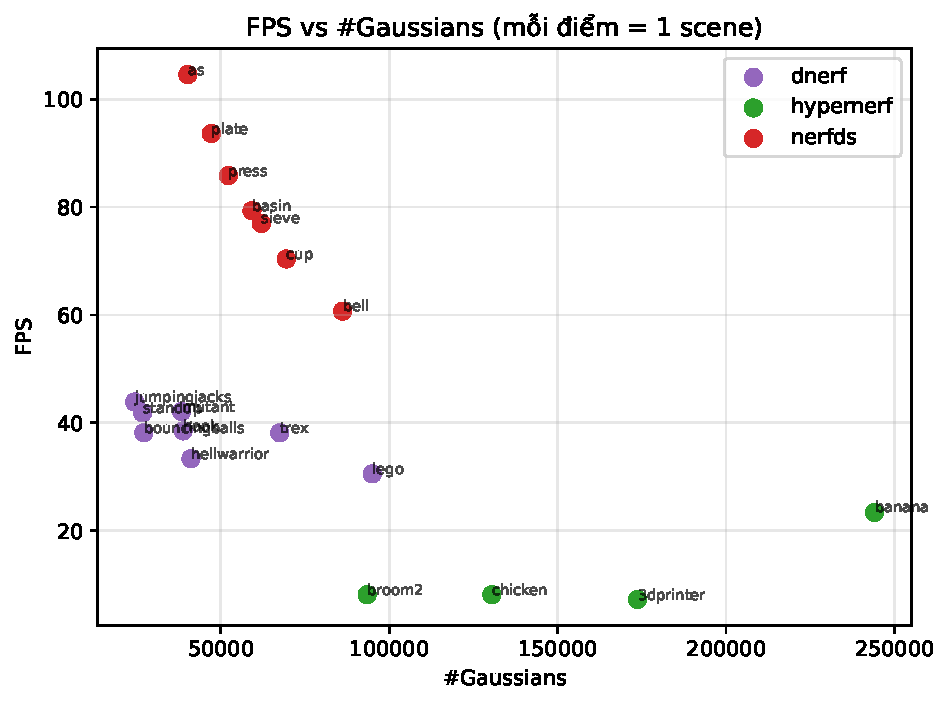
\includegraphics[width=\textwidth]{scatter_fps_gaussians}
    \caption{Quan hệ tốc độ render (FPS) và số Gaussian mỗi cảnh; mỗi điểm là một
    cảnh (cùng kiểu phân tích với hình point-FPS của bài báo gốc). FPS giảm khi số
    Gaussian tăng, lý giải vì sao cảnh quy mô lớn sẽ phá vỡ tính thời gian thực.}
    \label{fig:scatter}
\end{figure}

\chapter{Phân tích phản biện (Critical thinking)}
\label{chap:critical}

\section{Điểm mạnh}

Đóng góp giá trị nhất của 4D-GS là nó biến render cảnh động thời gian thực từ
một mục tiêu thành một thực tế kiểm chứng được. Sự khác biệt với các phương pháp
NeRF động không phải là vài chục phần trăm mà là hai bậc độ lớn: 82 FPS trên RTX
3090 so với dưới 3 FPS của TiNeuVox hay HexPlane trên cùng dữ liệu. Đáng nói hơn,
tính chất này không phụ thuộc phần cứng đầu bảng: trên chiếc T4 miễn phí của
Colab, nhóm vẫn đo được $\sim$30--44 FPS, đủ ngưỡng tương tác. Nguồn gốc của lợi thế
nằm ở quyết định kiến trúc phân tích tại chương~\ref{chap:method}: giữ nguyên pipeline splatting
và chỉ trả thêm đúng một lần truy vấn trường biến dạng mỗi khung hình.

Lợi thế thứ hai là tính gọn có cấu trúc. Một cảnh hoàn chỉnh chỉ chiếm khoảng
18 MB (10 MB Gaussian cộng 8 MB trường biến dạng) và con số này là hằng số theo
độ dài video, trong khi hướng Gaussian-mỗi-khung-hình phình tuyến tính. Kết hợp
với thời gian huấn luyện 11--20 phút mỗi cảnh (đo trên D-NeRF), chi phí tạo ra một biểu diễn 4D
trở nên rất thấp so với chuẩn mực của lĩnh vực chỉ một năm trước đó (HyperNeRF
cần 32 giờ huấn luyện cho chất lượng thấp hơn).

Về độ tin cậy khoa học, trải nghiệm thực nghiệm của nhóm cho điểm cộng rõ ràng:
toàn bộ 8 cảnh D-NeRF tái lập được \textit{chính xác đến mức trung bình trùng
khớp} (34,06 dB), và ngay cả trên dataset ngoài bài báo, kết quả vẫn khớp số đo
độc lập của bên thứ ba với sai số trung bình $\sim$0,5 dB. Một phương pháp mà người ngoài chạy
lại ra đúng số công bố là một phương pháp được công bố trung thực. Cuối cùng,
biểu diễn tường minh bằng các điểm Gaussian mở những khả năng mà biểu diễn hàm
ẩn khó với tới: bài báo trình diễn việc bám quỹ đạo điểm 3D và ghép nhiều cảnh
4D đã huấn luyện vào cùng một không gian render, hai thao tác gần như bất khả
thi với một MLP đen kín kiểu NeRF.

\section{Hạn chế}

Các hạn chế của 4D-GS có thể chia thành ba nhóm theo nguồn gốc. Nhóm thứ nhất
đến từ \textbf{giả định mô hình}. Thiết kế ``một bộ Gaussian chuẩn cộng biến
dạng trơn'' ngầm giả định cảnh là một khối hình học liên tục biến đổi; giả định
này gãy khi chuyển động đột ngột hoặc topology thay đổi (chất lỏng, khói, vật
xuất hiện rồi biến mất), thể hiện qua chính failure case chiếc chổi trong phụ
lục bài báo. Cùng nhóm này là phát hiện riêng của nhóm ở mục~\ref{sec:nerfds}:
vì màu SH của mỗi Gaussian cố định theo thời gian và bộ giải mã chỉ biến dạng
hình học, mọi hiệu ứng quang học động (phản xạ trượt trên vật bóng) nằm ngoài
không gian biểu diễn; hệ quả đo được là 17,8 dB trên cảnh \textit{plate}, và trên
NeRF-DS nói chung lợi thế chất lượng của 4D-GS không còn rõ: xếp sau các phương
pháp chuyên cho vật phản chiếu (mục~\ref{sec:nerfds}). Bài báo gốc
không đề cập hạn chế này.

Nhóm thứ hai đến từ \textbf{chế độ dữ liệu}. Phương pháp phụ thuộc mạnh vào
chất lượng khởi tạo hình học và camera pose: thiếu điểm nền hoặc pose nhiễu làm
tối ưu phân kỳ, như chính tác giả thừa nhận. Trong thiết lập đơn camera trên dữ
liệu thật, nhóm đo được khoảng cách train-test tới 12 dB trên NeRF-DS, một mức
overfitting cho thấy mô hình ``học thuộc'' các khung hình huấn luyện thay vì
nội suy được góc nhìn mới; trên dữ liệu thật nhiễu như HyperNeRF, chất lượng
cũng chỉ nhỉnh hơn TiNeuVox-B khoảng 0,8 dB (25,13 so với 24,3) trong khi huấn luyện lâu gấp đôi, tức lợi
thế thực chất chỉ còn ở tốc độ render. Phương pháp cũng chưa tách được phần
tĩnh và phần động của cảnh nếu thiếu giám sát bổ sung.

Nhóm thứ ba mang tính \textbf{kỹ thuật triển khai} nhưng ảnh hưởng thực tế không
nhỏ. Chi phí truy vấn trường biến dạng tỉ lệ với số Gaussian, nên với cảnh quy
mô đô thị hàng triệu điểm, tính thời gian thực sẽ vỡ; bản thân bài báo ghi nhận
tốc độ giảm rõ khi số điểm trong khung nhìn vượt 30.000. Ngoài ra, qua quá trình
áp dụng lên dataset mới, nhóm nhận thấy mã nguồn công bố hardcode một số tham
số theo dataset của bài báo (tỉ lệ downscale, đường dẫn point cloud), khiến
việc tái sử dụng đòi hỏi đọc-sửa code thay vì chỉ đổi cấu hình; với người dùng
không chuyên, đây là rào cản đáng kể và là lý do các con số ``chạy lại'' trong
cộng đồng dễ bị sai lệch một cách vô tình (như chính lần chạy đầu của nhóm bị
thổi phồng PSNR do độ phân giải).

\section{Khả năng áp dụng thực tế}

Hồ sơ năng lực của 4D-GS (huấn luyện khoảng 10 phút đến hơn một giờ mỗi cảnh, model 18 MB, render
30+ FPS trên GPU phổ thông) định vị nó vào các ứng dụng \textit{quay trước, xem
lại tương tác}. Trong sản xuất phim và quảng cáo, một cảnh quay đa góc máy có
thể được huấn luyện trong giờ nghỉ trưa rồi cho đạo diễn ``bay camera'' tự do
quanh khoảnh khắc đã quay, thay thế các dàn bullet-time hàng trăm máy ảnh. Trong
thể thao và biểu diễn, mô hình đủ nhẹ để phân phối tới thiết bị người xem
như một định dạng ``video 4D''. Với VR cần lưu ý ngưỡng khắt khe hơn: kính VR
đòi hỏi 72--90 FPS cho mỗi mắt, nên T4 ($\sim$30--44 FPS một mắt) chưa đủ mà cần GPU
cỡ RTX 3090 hoặc giảm độ phân giải.

Ở chiều ngược lại, ba đặc tính loại 4D-GS khỏi nhiều kịch bản. Nó là mô hình
\textit{per-scene}, mỗi cảnh huấn luyện riêng và không tổng quát hóa, nên không
phù hợp dựng cảnh tức thời từ video streaming (hội nghị truyền hình 3D thời gian
thực). Nó cần pose camera chính xác, thường từ COLMAP, nên video quay tay tùy
tiện không qua tiền xử lý cẩn thận sẽ thất bại. Và như kết quả NeRF-DS cho thấy,
các môi trường nhiều bề mặt phản chiếu (showroom, nhà bếp, sản phẩm kim loại
trong quảng cáo) chính là vùng rủi ro chất lượng cao nhất.

\section{Khi nào phương pháp hoạt động tốt / có thể thất bại}

Từ phân tích phương pháp và các thí nghiệm trên ba dataset, nhóm rút ra quy luật:
chất lượng của 4D-GS tỉ lệ thuận với mức độ ``hình học hóa được'' của cảnh.
Phương pháp hoạt động tốt khi cảnh có ranh giới rõ, chuyển động biên độ vừa
phải và trơn theo thời gian (người cử động, vật rơi/nảy, đúng như 8 cảnh D-NeRF
đạt 25--41 dB), khi có nhiều góc máy hoặc camera quỹ đạo bao quanh đối tượng với
pose chính xác, và khi bề mặt vật thể khuếch tán (diffuse) để màu cố định theo
thời gian là xấp xỉ hợp lệ.

Ngược lại, có thể dự đoán thất bại khi một trong các điều kiện trên bị vi phạm:
chuyển động đột ngột biên độ lớn vượt quá độ trơn mà lưới HexPlane cộng TV loss
áp đặt (failure case chiếc chổi); pose nhiễu hoặc thiếu điểm nền làm gãy khâu
khởi tạo; bề mặt phản chiếu mạnh khiến giả định màu tĩnh sụp đổ (cảnh
\textit{plate} của nhóm); topology thay đổi khiến không tồn tại bộ Gaussian
chuẩn nào nhất quán với mọi thời điểm; và cảnh quy mô lớn khiến chi phí truy vấn
trường biến dạng nuốt mất ngân sách thời gian thực. Điểm đáng giá của khung phân
tích này là nó \textit{dự đoán được}: nhóm đã dùng nó để chọn cặp cảnh
sieve/plate trước khi chạy, và kết quả thực nghiệm xác nhận đúng cả hai chiều.

% ============================================================
% CHƯƠNG 5 — KẾT LUẬN
% ============================================================
\chapter{Kết luận}

Báo cáo đã tìm hiểu bài báo 4D Gaussian Splatting (CVPR 2024): bài toán render
cảnh động thời gian thực, phương pháp biểu diễn một bộ Gaussian chuẩn kết hợp
trường biến dạng HexPlane, và các đóng góp chính. Nhóm chạy lại mã nguồn chính
thức trên Google Colab (T4) và áp dụng lên \textbf{ba dataset}. Trên hai bộ của
bài báo, kết quả tái lập đúng: D-NeRF (8 cảnh tổng hợp) đạt PSNR trung bình
34,06 dB \textbf{trùng khớp số công bố}, HyperNeRF (4 cảnh thật) cũng sát số công
bố, xác nhận tính tái lập trên cả dữ liệu tổng hợp lẫn thật; tốc độ render
$\sim$30--44 FPS trên T4 xác nhận tính thời gian thực ngay trên phần cứng phổ thông.

Nhóm cũng áp dụng phương pháp lên \textbf{NeRF-DS} (vật phản chiếu, ngoài bài báo)
và tổng hợp \textbf{so sánh chéo ba dataset}: chất lượng 4D-GS giảm dần theo trục
tổng hợp $\to$ thật khuếch tán $\to$ thật phản chiếu, trong khi đặc tính tốc độ và
độ gọn giữ ổn định. Quá trình này phơi bày hai hạn chế chưa được nêu trong bài báo
gốc: kém với vật liệu phản chiếu (do màu SH cố định theo thời gian) và overfitting
trong thiết lập đơn camera. Phân tích phản biện chỉ ra phương pháp mạnh ở tốc độ,
độ gọn và khả năng thao tác trên biểu diễn tường minh, nhưng còn hạn chế với chuyển
động lớn, cảnh quy mô lớn, vật liệu phản chiếu và thiết lập đơn camera thiếu giám
sát. Hướng phát triển tự nhiên là trường biến dạng gọn hơn cho cảnh đô thị, cơ chế
tách tĩnh/động không cần giám sát, và mô hình hóa thành phần phản xạ biến đổi theo
thời gian.

% ============================================================
% ĐÓNG GÓP THÀNH VIÊN
% ============================================================
\chapter*{Đóng góp các thành viên trong nhóm}
\addcontentsline{toc}{chapter}{Đóng góp thành viên}

\resizebox{\textwidth}{!}{%
\begin{tabular}{|p{37mm}|p{20mm}|p{72mm}|p{25.6mm}|}
\hline
\textbf{Sinh viên} & \textbf{MSSV} & \textbf{Tác vụ thực hiện} & \textbf{Đóng góp (\%)} \\
\hline
Ngô Văn Minh Thắng & 20020155 & Chạy thực nghiệm 4D-GS trên ba dataset D-NeRF, HyperNeRF, NeRF-DS (Google Colab); xử lý lỗi tương thích môi trường; tổng hợp số liệu, biểu đồ; biên soạn báo cáo LaTeX; viết Chương 3 (Kết quả thực nghiệm) và Chương 5 (Kết luận) & \\
\hline
Trần Trọng Thịnh & 22028073 & Nghiên cứu và tóm tắt bài báo gốc; viết Chương 1 (Giới thiệu) và Chương 2 (Phương pháp); làm slide trình bày & \\
\hline
Nguyễn Xuân Anh & 22028257 & Viết Chương 4 (Phân tích phản biện); làm slide trình bày; rà soát và hoàn thiện báo cáo & \\
\hline
\end{tabular}%
}

% ============================================================
% LINK SOURCE CODE
% ============================================================
\chapter*{Link Source code của nhóm}
\addcontentsline{toc}{chapter}{Link Source code}

Repo chứa notebook thực nghiệm (kèm log huấn luyện đầy đủ), kết quả các cảnh
(metrics, ảnh render/ground-truth, video) và mã nguồn bài báo dưới dạng submodule:

\textbf{Link Source code:}
\href{https://github.com/MinhThang1009/computer-vision}{github.com/MinhThang1009/computer-vision}

\textbf{Link Notebook Colab (chạy trực tiếp):}
\href{https://colab.research.google.com/drive/1R94YpYTDryfU0K0t1xjnxTq4uJK2xlvV}{Mở notebook trên Google Colab}

\textbf{Link Google Drive (kết quả: output, reports, figures):}
\href{https://drive.google.com/drive/folders/1jA0eAe2oQbptRWEgGnqoMk1K-1dy0Wuk}{Thư mục kết quả trên Google Drive}

% ============================================================
% TÀI LIỆU THAM KHẢO
% ============================================================
\begin{thebibliography}{14}
\addcontentsline{toc}{chapter}{Tài liệu tham khảo}

\bibitem{wu20244dgs}
G. Wu, T. Yi, J. Fang, L. Xie, X. Zhang, W. Wei, W. Liu, Q. Tian, X. Wang.
\href{https://arxiv.org/pdf/2310.08528}{4D Gaussian Splatting for Real-Time Dynamic Scene Rendering}.
\textit{CVPR}, 2024.

\bibitem{3dgs}
B. Kerbl, G. Kopanas, T. Leimkühler, G. Drettakis.
\href{https://arxiv.org/pdf/2308.04079}{3D Gaussian Splatting for Real-Time Radiance Field Rendering}.
\textit{ACM Transactions on Graphics}, 42(4), 2023.

\bibitem{mildenhall2021nerf}
B. Mildenhall, P. P. Srinivasan, M. Tancik, J. T. Barron, R. Ramamoorthi, R. Ng.
\href{https://arxiv.org/pdf/2003.08934}{NeRF: Representing Scenes as Neural Radiance Fields for View Synthesis}.
\textit{ECCV}, 2020.

\bibitem{pumarola2021dnerf}
A. Pumarola, E. Corona, G. Pons-Moll, F. Moreno-Noguer.
\href{https://arxiv.org/pdf/2011.13961}{D-NeRF: Neural Radiance Fields for Dynamic Scenes}.
\textit{CVPR}, 2021.

\bibitem{kplanes}
S. Fridovich-Keil, G. Meanti, F. R. Warburg, B. Recht, A. Kanazawa.
\href{https://arxiv.org/pdf/2301.10241}{K-Planes: Explicit Radiance Fields in Space, Time, and Appearance}.
\textit{CVPR}, 2023.

\bibitem{hexplane}
A. Cao, J. Johnson.
\href{https://arxiv.org/pdf/2301.09632}{HexPlane: A Fast Representation for Dynamic Scenes}.
\textit{CVPR}, 2023.

\bibitem{tineuvox}
J. Fang, T. Yi, X. Wang, L. Xie, X. Zhang, W. Liu, M. Nießner, Q. Tian.
\href{https://arxiv.org/pdf/2205.15285}{Fast Dynamic Radiance Fields with Time-Aware Neural Voxels}.
\textit{SIGGRAPH Asia}, 2022.

\bibitem{guo2023forwardflowfornvs}
X. Guo, J. Sun, Y. Dai, G. Chen, X. Ye, X. Tan, E. Ding, Y. Zhang, J. Wang.
\href{https://arxiv.org/pdf/2309.17390}{Forward Flow for Novel View Synthesis of Dynamic Scenes}.
\textit{ICCV}, 2023.

\bibitem{msth}
F. Wang, Z. Chen, G. Wang, Y. Song, H. Liu.
\href{https://arxiv.org/pdf/2310.17527}{Masked Space-Time Hash Encoding for Efficient Dynamic Scene Reconstruction}.
\textit{NeurIPS}, 2023.

\bibitem{yan2023nerfds}
Z. Yan, C. Li, G. H. Lee.
\href{https://arxiv.org/pdf/2303.14435}{NeRF-DS: Neural Radiance Fields for Dynamic Specular Objects}.
\textit{CVPR}, 2023.

\bibitem{park2021hypernerf}
K. Park, U. Sinha, P. Hedman, J. T. Barron, S. Bouaziz, D. B. Goldman, R. Martin-Brualla, S. M. Seitz.
\href{https://arxiv.org/pdf/2106.13228}{HyperNeRF: A Higher-Dimensional Representation for Topologically Varying Neural Radiance Fields}.
\textit{ACM Transactions on Graphics (SIGGRAPH Asia)}, 2021.

\bibitem{spectromotion}
C.-D. Fan, Y.-C. Sun, J.-H. Wu, B.-Y. Wang, S.-Y. Chen, et al.
\href{https://arxiv.org/pdf/2410.17249}{SpectroMotion: Dynamic 3D Reconstruction of Specular Scenes}.
\textit{CVPR}, 2025.

\bibitem{dynamic3dgs}
J. Luiten, G. Kopanas, B. Leibe, D. Ramanan.
\href{https://arxiv.org/pdf/2308.09713}{Dynamic 3D Gaussians: Tracking by Persistent Dynamic View Synthesis}.
\textit{3DV}, 2024.

\bibitem{deformable3dgs}
Z. Yang, X. Gao, W. Zhou, S. Jiao, Y. Zhang, X. Jin.
\href{https://arxiv.org/pdf/2309.13101}{Deformable 3D Gaussians for High-Fidelity Monocular Dynamic Scene Reconstruction}.
\textit{CVPR}, 2024.

\end{thebibliography}

\end{document}
